% Do not forget to include Introduction
%---------------------------------------------------------------
% \chapter{Introduction}
% uncomment the following line to create an unnumbered chapter
\chapter*{Úvod}\addcontentsline{toc}{chapter}{Úvod}\markboth{Úvod}{Úvod}
%---------------------------------------------------------------
\setcounter{page}{1}

% The following environment can be used as a mini-introduction for a chapter. Use that any way it pleases you (or comment it out). It can contain, for instance, a summary of the chapter. Or, there can be a quotation.
\begin{chapterabstract}
	\lipsum[1]
\end{chapterabstract}

\lipsum[4]

%---------------------------------------------------------------
\section{Vzory}
%---------------------------------------------------------------

%---------------------------------------------------------------
\subsection{List}
%---------------------------------------------------------------

\begin{itemize}
    \item Ut enim ad minim veniam, quis nostrud
    \item Ut enim ad minim 
    \begin{itemize}
        \item Ut enim ad
        \item Ut enim ad
    \end{itemize}
\end{itemize}

%---------------------------------------------------------------
\subsection{Číslovaný list}
%---------------------------------------------------------------

\begin{enumerate}
    \item Ut enim ad minim veniam, quis nostrud
    \item Ut enim ad minim 
    \begin{enumerate}
        \item Ut enim ad
        \item Ut enim ad
    \end{enumerate}
\end{enumerate}

%---------------------------------------------------------------
\subsection{Kód}
%---------------------------------------------------------------

\vspace{\baselineskip} 
\begin{lstlisting}[caption={~Zbytočný kód},label=list:8-6,captionpos=t,abovecaptionskip=-\medskipamount,belowcaptionskip=\medskipamount,language=C]
    #include<stdio.h>
    #include<iostream>
    // A comment
    int main(void)
    {
        printf("Hello World\n");
        return 0;
    }
\end{lstlisting}

%---------------------------------------------------------------
\subsection{Tabuľka}
%---------------------------------------------------------------

\begin{table}[h!]\centering
\caption[Příklad tabulky]{~Zadávání matematiky}\label{tab:matematika}
\begin{tabular}{l|l|c|c}
	Typ		& Prostředí		& \LaTeX{}ovská zkratka	& \TeX{}ovská zkratka	\tabularnewline \hline 
 	Text		& \verb|math|		& \verb|\(...\)|	& \verb|$...$|	\tabularnewline \hline
 	Displayed	& \verb|displaymath|	& \verb|\[...\]|	& \verb|$$...$$|	\tabularnewline 
\end{tabular}
\end{table}

\subsection{Dôkazy}

\begin{definition}[Optional label]
Class aptent taciti sociosqu ad litora torquent per conubia nostra, per inceptos hymenaeos. Fusce suscipit libero eget elit. Etiam dui sem, fermentum vitae, sagittis id, malesuada in, quam. Aliquam id dolor. Curabitur bibendum justo non orci.
\end{definition}

\begin{example}
Class aptent taciti sociosqu ad litora torquent per conubia nostra, per inceptos hymenaeos. Fusce suscipit libero eget elit. Etiam dui sem, fermentum vitae, sagittis id, malesuada in, quam. Aliquam id dolor. Curabitur bibendum justo non orci.
\end{example}

\begin{theorem}
Class aptent taciti sociosqu ad litora torquent per conubia nostra, per inceptos hymenaeos. Fusce suscipit libero eget elit. Etiam dui sem, fermentum vitae, sagittis id, malesuada in, quam. Aliquam id dolor. Curabitur bibendum justo non orci.
\end{theorem}

\begin{proof}
Fusce suscipit libero eget elit. Etiam dui sem, fermentum vitae, sagittis id, malesuada in, quam. Aliquam id dolor. Curabitur bibendum justo non orci.
\end{proof}

\begin{corollary}
Fusce suscipit libero eget elit. Etiam dui sem, fermentum vitae, sagittis id, malesuada in, quam. Aliquam id dolor. Curabitur bibendum justo non orci.
\end{corollary}




%---------------------------------------------------------------
\chapter{Analýza problému}
%---------------------------------------------------------------

%---------------------------------------------------------------
\section{Stavba a funkcia srdca}
%---------------------------------------------------------------

Srdce je svalový orgán, ktorý sa nachádza v ľavej časti ľudského hrudníka, kde je chránený hrudným košom. Je zodpovedný za pumpovanie krvi do celého tela, čím rozvádza kyslík do jednotlivých orgánov a tkanív. Z hľadiska anatómie je srdečná dutina rozdelená priehradkami na ľavé a pravé srdce. Tie sú potom každé rozdelené na dve ďalšie časti - pravú a ľavú predsieň, a pravú a ľavú komoru. Do pravej predsiene prúdi odkysličená krv z tela cez hornú a dolnú dutú žilu, z kade ďalej tečie cez trikuspidálnu trojcípu chlopňu do pravej komory. Tá následne krv pumpuje cez pľúcne tepny do pľúc na okysličenie. Naopak do ľavej predsiene tečie cez pľúcne žily okysličená krv, kde následne prúdi cez mitrálnu dvojcípu chlopňu do ľavej komory, z kade sa dostáva cez aortu do krvného obehu.\cite{Weinhaus}\cite{Britannica_2024}

Dráždivé tkanivo, z ktorého je srdečný sval tvorený, je charakteristické \textbf{excitabilitou}, teda schopnosťou reagovať na elektrické impulzy. Svalovina srdca, alebo myokard, umožňuje rytmické kontrakcie srdca - \textbf{systolu a diastolu}. Pod systolou rozumieme časť srdečného rytmu kedy sa srdečný sval sťahuje, a vytláča tak krv z komôr do tepien. Primárne zahŕňa kontrakciu komôr, ktorá vedie k prúdeniu krvi do systémového obehu. Časť srdečného rytmu, kedy dochádza k relaxácii srdečného svalu a následnému naplneniu srdca krvou, sa nazýva diastola. Komory sa v tomto bode uvoľnia, čo umožní prúdenie novej krvi z predsiení.\cite{Weinhaus}

\begin{figure}[t]
    \centering
    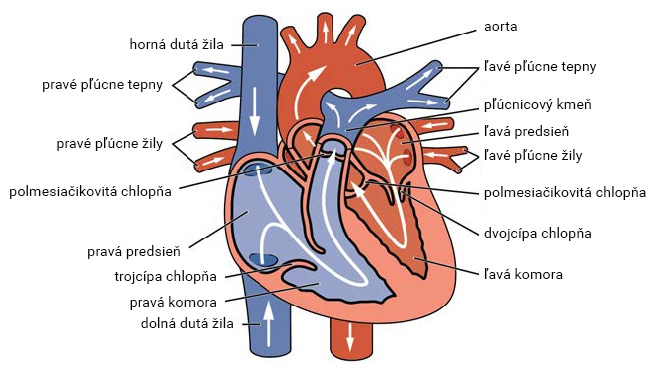
\includegraphics[scale=0.6]{img/srdce.jpg}
    \caption{Anatómia ľudského srdca\cite{Pančík_2016}}
\end{figure}

%---------------------------------------------------------------
\subsection{Akčný potenciál srdcovej membrány}
%---------------------------------------------------------------

 Elektrické impulzy, na ktoré bunky srdečného svalu reagujú, spontánne vznikajú v špecializovaných bunkách srdca - tie sa nazývajú kardiostimulátorové bunky. Počas srdečného cyklu bunky tvoriace srdce prechádzajú z \textbf{polarizovaného} stavu, teda pokojového, do stavu \textbf{depolarizovaného}, teda excitovaného. V polarizovanom stave dosahuje pokojový elektrický potenciál medzi povrchom a vnútrom bunky -90 mV.\cite{Bada2010} Elektrický stimul vyvoláva akčný potenciál, ktorý sa dá rozdeliť na päť fáz:
\begin{itemize}
    \item \textbf{Fáza 0} - depolarizácia v dôsledku prudkej zmeny polarity bunkovej membrány. Následkom je nárast akčného potenciálu až na 30mV.
    \item \textbf{Fáza 1} - prvotná repolarizácia, v tomto bode začína akčný potenciál klesať.
    \item \textbf{Fáza 2} - nazývaná aj plató, ide o dlhší interval, v ktorom sa polarita bunkovej membrány stabilne blíži k nule. Akčný potenciál je vďaka tejto fáze výrazne dlhší a umožňuje tak trvácnu kontrakciu srdcového svalu.
    \item \textbf{Fáza 3} - repolarizácia v dôsledku prudkej zmeny polarity bunkovej membrány. Bunka sa vracia do polarizovaného stavu.
    \item \textbf{Fáza 4} - interval medzi dvoma akčnými potenciálmi, kedy bunková membrána dosahuje pokojový elektrický potenciál. 
\end{itemize}

Jednotlivé fázy akčného potenciálu sú ilustrované na obrázku \ref{fig:action_potential_voltage}, kde je v čase zobrazená hodnota akčného potenciálu srdcovej membrány.\cite{Rooke2021TheEA}\cite{Bada2010}

\begin{figure}[H]
    \centering
    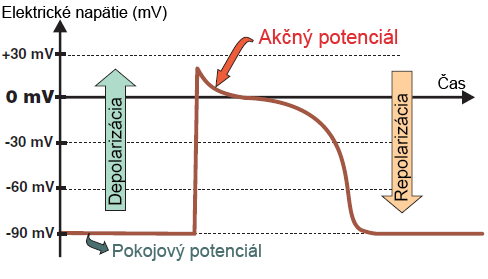
\includegraphics[scale=0.45]{img/action-potential-voltage.png}
    \caption{Akčný potenciál srdcovej membrány\cite{Blahút_2017}}
    \label{fig:action_potential_voltage}
\end{figure}


%---------------------------------------------------------------
\section{Elektrokardiografia}
%---------------------------------------------------------------

Proces získavania elektrokardiogramu (EKG) nazývame elektrokardiografia. Práve vyššie uvedený jednoduchý popis anatómie a fungovania ľudského srdca je kľúčový pre správnu interpretáciu vzniku EKG. "Elektrokardiografia je metóda, ktorá zaznamenáva elektrickú aktivitu srdca v čase. Zmeny v rozdiele elektrického potenciálu, teda napätí, ktoré vznikajú počas depolarizácie a repolarizácie myokardiálnych vlákien, sú zaznamenávané elektródami umiestnenými na povrchu hrudníka a končatinách. Zdrojom týchto elektrických potenciálov sú kontraktilné bunky srdcového svalu (kardiomyocity)."\footnote{Pôvodné znenie: \textit{"Electrocardiography is a method that registers electrical activity against time. The changes in electrical potential difference (voltage) during depolarization and repolarisation of the myocardial fibers are recorded by electrodes positioned on the surface of the chest and on the limb (limb leads). The sources of the electrical potentials are contractile cardiac muscle cells (cardiomyocytes)."}}\cite{Wasilewski2011}

V tejto práci sa budeme venovať prevažne záťažovej elektrokardiografii, nazývanej aj \textbf{ergometria}. Aj keď je princíp zaznamenávania EKG ten istý, toto vyšetrenie nesie so sebou určité špecifiká, najmä ak je vykonávané v teréne, čo je tiež prípad tejto práce. Keďže sa zaznamenáva srdečná aktivita pri fyzickej činnosti, nie je možné, aby mala na sebe sledovaná osoba štandardne umiestnené elektródy. Často musí byť použitý aj iný druh elektród, k tomu sa ale bližšie dostaneme v nasledujúcej časti práce.

Vykresľovanie aj interpretácia EKG krivky stále bežne prebieha v tlačenej forme na milimetrovom papieri, preto sú napríklad fyziologické intervaly, najmä v medicínskej literatúre, často uvádzané v milimetroch. Pre technický charakter tejto práce budeme hodnoty popisujúce dĺžku trvania uvádzať v časových jednotkách, najčastejšie milisekundách (ms). Amplitúdu krivky budeme popisovať v jednotkách elektrického napätia, v prípade EKG konkrétne v milivoltoch (mV). 

%---------------------------------------------------------------
\subsection{Elektródy a zvody}
%---------------------------------------------------------------

Na meranie zmien napätia v srdečnom elektrickom poli sa používajú rôzne druhy elektród, ktoré si bližšie opíšeme. Z hľadiska funkčnosti rozlišujeme pri EKG dva druhy. \textbf{Aktívne elektródy} merajú meniaci sa elektrický potenciál na mieste, na ktorom sú umiestnené. Druhým typom sú \textbf{referenčné alebo nulové elektródy}, ktoré udržiavajú stabilný potenciál, zvyčajne nulový. Spojením dvoch elektród vzniká zvod - imaginárna línia pozdĺž ktorej je meraný elektrický signál. Zvody klasifikujeme na \textbf{bipolárne} a \textbf{unipolárne}. Bipolárne zvody sa skladajú z dvoch aktívnych elektród, zatiaľ čo unipolárne zvody z jednej aktívnej elektródy a jednej nulovej. Pri elektrokardiografickom vyšetrení vykonávanom v ambulancii sa EKG zaznamenáva pomocou štandardizovaného 12-zvodového systému, ktorý má predpísané rozloženie elektród.

%---------------------------------------------------------------
\subsection{Einthovenove končatinové zvody}
%---------------------------------------------------------------

Prvé tri zvody využívané pri 12-zvodovom EKG sú Einthovenove končatinové zvody. Ide o bipolárne zvody, na získanie ktorých potrebujeme 4 elektródy - na ľavej hornej končatine (ĽR), pravej hornej končatine (PR), ľavej dolnej končatine (ĽN) a pravej dolnej končatine (PN). Elektróda na pravej dolnej končatine je nulová, ostatné sú aktívne. Tieto elektródy sa zvyčajne umiestňujú na predlaktie a predkolenie, na presnom umiestnení však nezáleží, je iba potrebné zabezpečiť vzdialenosť minimálne 10 centimetrov od srdca.\cite{garcia201512} Zvody, ktoré vzniknú spojením týchto elektród, označujeme rímskymi číslicami.

\begin{itemize}
    \item \textbf{I. štandardný zvod} - získame ho ako rozdiel potenciálov medzi elektródami na ľavom a pravom predlaktí.
    \item \textbf{II. štandardný zvod} - 
    získame ho ako rozdiel potenciálov medzi elektródami na pravom predlaktí a ľavom predkolení.
    \item \textbf{III. štandardný zvod} - 
     získame ho ako rozdiel potenciálov medzi elektródami na ľavom predlaktí a ľavom predkolení.\cite{Bada2010}
\end{itemize}

"Štandardné končatinové zvody snímajú srdcové potenciály vo frontálnej rovine. Spojením troch štandardných zvodov vzniká \textbf{rovnostranný Einthovenov trojuholník}, v ktorého približnom strede sa nachádza srdce - v polohe ako sa nachádza v hrudníku."\cite{Bada2010} Tento trojuholník sa používa aj na určenie elektrickej osi srdečnej, ktorou sa ešte budeme zaoberať neskôr v práci.

\begin{figure}[H]
    \centering
    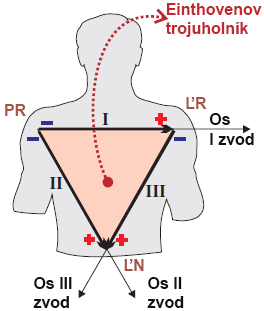
\includegraphics[scale=0.6]{img/einthoven-triangle.png}
    \caption{Einthovenove končatinové zvody\cite{Blahút_2017a}}
    \label{fig:einthoven}
\end{figure}

%---------------------------------------------------------------
\subsection{Goldbergove končatinové zvody}
%---------------------------------------------------------------

Ďalšie zvody zaznamenávané pri 12-zvodovom EKG sú Goldbergove končatinové zvody. Opäť ide o tri zvody, v tomto prípade ale unipolárne - každý je kombináciu jednej aktívnej a jednej nulovej elektródy. Na ich získanie sa využívajú potenciály z tých istých elektród ako pri Einthovenových zvodoch. Nulová elektróda sa získava prepojením ostatných dvoch, čím sa potenciál aktívnej elektródy umelo zvýši. Od tejto skutočnosti je odvodený aj pojem \textbf{augmentovaný zvod} a značenie aV (\textit{a = augmented = zvýšené} a \textit{V = voltage = napätie}). Tretie písmeno za skratkou aV značí pozíciu aktívnej elektródy.

\begin{itemize}
    \item \textbf{aVR} - aktívna elektróda je umiestnená na pravom predlaktí, záznam je prevráteným obrazom I. štandardného zvodu.
    \item \textbf{aVL} - aktívna elektróda je umiestnená na ľavom predlaktí, záznam pri tomto zvode sa podobá na I. štandardný zvod.
    \item \textbf{aVF} - aktívna elektróda je umiestnená na ľavom predkolení, záznam pri tomto zvode sa podobá na III. štandardný zvod.\cite{Bada2010}\cite{garcia201512} 
\end{itemize}

\begin{figure}[H]
    \centering
    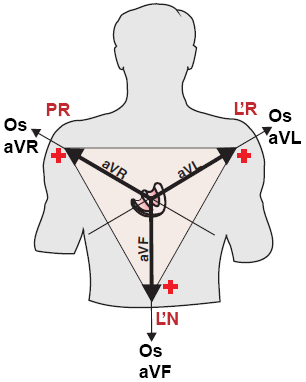
\includegraphics[scale=0.5]{img/goldberger-leads.png}
    \caption{Goldbergove končatinové zvody\cite{Blahút_2017a}}
    \label{fig:goldberg}
\end{figure}

%---------------------------------------------------------------
\subsection{Wilsonove hrudné zvody}
%---------------------------------------------------------------

Zvyšných šesť zvodov sa nachádza na hrudníku, nazývajú sa Wilsonove zvody. Všetky zvody sú unipolárne a označujú sa V1 až V6. Na rozdiel od elektród využívaných predošlými Einthovenovými a Goldbergovými zvodmi majú tieto elektródy presne určenú pozíciu, ktorá je definovaná polohou jednotlivých rebier.\cite{Bada2010}\cite{garcia201512} Predpísané polohy jednotlivých elektród nebudeme bližšie rozpisovať, ilustrované sú na obrázku \ref{fig:wilson}.

Hrudné zvody snímajú elektrickú aktivitu srdca v horizontálnej rovine. "Tvar krivky EKG zaznamenaný pomocou unipolárnych hrudných zvodov determinuje vzájomný vzťah polohy snímajúcej elektródy k smeru šírenia sa vzruchu v srdci. Vzruch v srdci sa šíri smerom od sínusového uzla v pravej predsieni k srdcovému hrotu."\cite{Bada2010}

\begin{figure}[H]
    \centering
    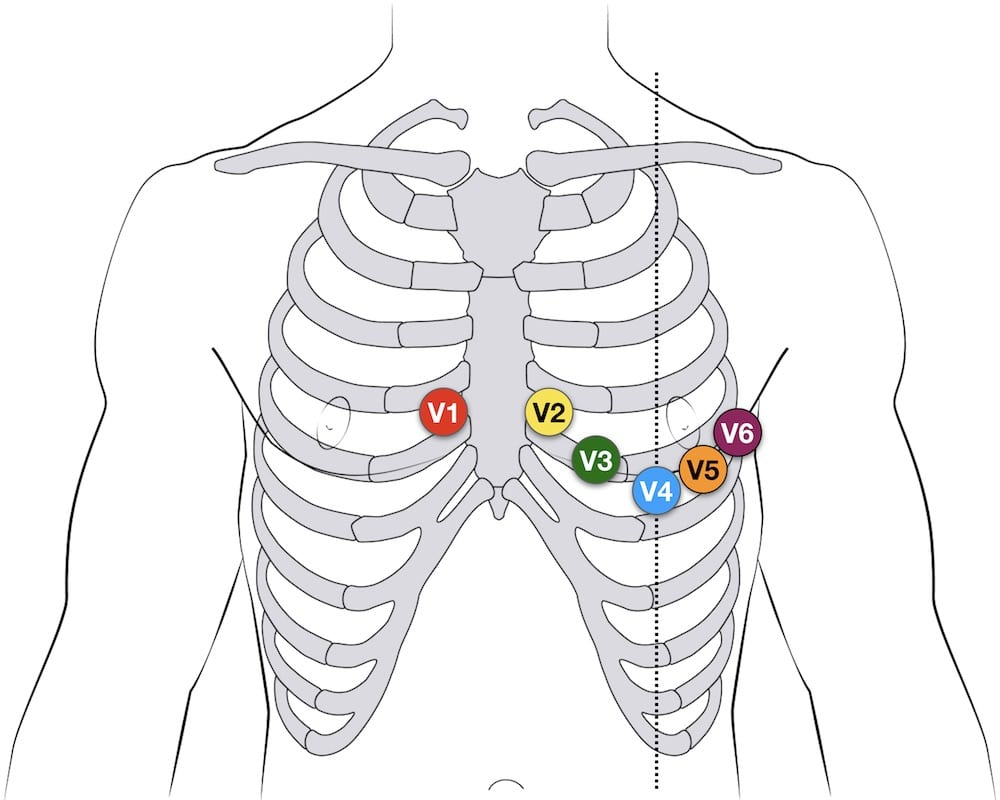
\includegraphics[scale=0.25]{img/12-lead-ECG-lead-placemnet.jpg}
    \caption{Wilsonove hrudné zvody\cite{Cadogan_2022}}
    \label{fig:wilson}
\end{figure}

Dôležité je spomenúť, že pri dlhodobom terénnom monitorovaní sa často využíva 1-zvodový systém, na ktorý sú potrebné iba 3 elektródy. Tie sú často umiestnené práve na hrudníku - prvá elektróda na jednom z miest V1 až V6, druhá zrkadlovo na druhej polovici hrudníka, a tretia pod ich úrovňou, v oblasti brucha. Takýmto spôsobom sa minimalizuje počet použitých elektród a káblov potrebných na ich zapojenie, čo je pri dlhodobom monitorovaní prioritou.\cite{Thakor1980}


%---------------------------------------------------------------
\section{Typy povrchových elektród}
%---------------------------------------------------------------

Elektródy používané v elektrokardiografii vieme rozdeliť na povrchové a hĺbkové elektródy. Ako aj samotné názvy napovedajú, povrchové elektródy sa umiestňujú na povrch tela, teda na kožu, zatiaľ čo hĺbkové elektródy sa aplikujú priamo do srdečného svalu. Pre účely tejto práce nás budú zaujímať iba povrchové elektródy, hĺbkové majú svoje miesto v medicíne najmä pri operatívnych zákrokoch. 

Použitie vhodného typu povrchových elektród je rozhodujúce pre kvalitu výsledného EKG záznamu. Ako už bolo vyššie spomenuté, rôzne situácie si vyžadujú rôzne druhy elektród. "Keďže EKG je záznam bio elektrických potenciálov na povrchu tela, rozhranie medzi kožou pacienta a elektródami zaznamenávajúcimi EKG je kritické. Významná časť artefaktov zavedených do EKG záznamov sa vyskytuje práve na tomto rozhraní a je spôsobená buď neadekvátnou prípravou kože, alebo nedostatočným kontaktom medzi kožou a elektródou."\footnote{Pôvodné znenie: \textit{"As the ECG is a recording of bioelectrical potentials made at the body surface, the interface between the patient’s skin and the recording electrodes of the ECG is critical. Much of the artifact introduced into ECG recordings occurs at this junction and is caused by inadequate skin preparation or in- adequate skin–electrode contact."}}\cite{Garvey2006} V nasledujúcej časti si predstavíme dva bežné typy povrchových elektród, so zameraním na terénnu záťažovú elektrokardiografiu.

%---------------------------------------------------------------
\subsection{Argentchloridové elektródy}
%---------------------------------------------------------------

Súčasne najpoužívanejším druhom elektród v medicíne sú tradičné argentchloridové elektródy, skrátene Ag/AgCl elektródy. "Ich názov pochádza od chloridu strieborného AgCl - argentchloridu, sú základom nie len referenčných elektród pre najrôznejšie analytické systémy, ale zároveň základom väčšiny elektród určených pre snímanie biologických signálov na povrchu tela."\cite{Roubík2007} Kovová časť tejto elektródy sa skladá zo striebra, na povrchu ktorého je vrstva chloridu strieborného. Ako elektrolyt, teda materiál ktorý zabezpečí vedenie elektrického prúdu, sa pri týchto elektródach v medicíne používa fyziologický roztok.\cite{Roubík2007}

Jednou z výhod Ag/AgCl elektród je nízka impedancia, teda kladenie minimálneho odporu elektrickému prúdu, kvôli čomu je signál zachytený týmito elektródami dostatočne presný. Ďalšou dôležitou výhodou je pevný kontakt s kožou pacienta, ktorý zaručuje spoľahlivý prenos elektrického signálu aj pri pohybe. Tieto elektródy majú samozrejme aj nevýhody, ktoré sú najvýznamnejšie práve pri terénnom a dlhodobom monitorovaní. Bežná Ag/AgCl elektróda je určená len na jedno použitie a odporučená doba skladovania je menej ako jeden rok, po odlepení, či vypršaní doby skladovania, prichádza o svoje pozitívne vlastnosti.\cite{Marozas2011} Z hľadiska dlhodobého monitorovania predstavuje tento typ elektród tiež problém. "Dlhodobé monitorovanie pomocou týchto elektród nie je vhodné, lebo bunky stratum corneum (vonkajšej vrstvy kože) sa v priebehu 24 hodín regenerujú a abrazívny efekt zmizne. Dráždenie pokožky je navyše nepríjemné a ak sú elektródy použité v kombinácii s gélmi, riziko podráždenia pokožky výrazne stúpa. V neposlednom rade ide aj o nepohodlie súvisiace s osobnou hygienou, keďže s nalepenými elektródami sprchovanie nie je možné."\footnote{Pôvodné znenie: \textit{"This measure is not suitable for long-term monitoring because the cells of stratum corneum (outermost layer of the skin) regenerate from deeper skin layers during 24 hours, and the abrasion effect disappears; also, skin abrasion is unpleasant and, if used together with gels, significantly increases the risk of skin irritation. Finally, there is also the personal inconvenience of not being able to shower or bathe while using the electrodes. "}}\cite{Marozas2011}

%---------------------------------------------------------------
\subsection{Textilné elektródy}
%---------------------------------------------------------------

Za posledné roky dostupnosť inteligentných nositeľných zariadení rapídne rastie, spolu s čím výrazne napreduje aj výskum v oblasti využitia textilných elektród. Tie nie sú primárne určené na ambulantné monitorovanie, ale na terénne monitorovanie pri stresových a fyzicky náročných profesiách, akými sú napríklad rôzne zásahové zložky, prípadne na voľnočasové monitorovanie pri športových aktivitách. Textilné elektródy sú väčšinou integrované do oblečenia, alebo do hrudného pásu, a najčastejšie sa využíva 1-zvodový EKG systém s troma elektródami.\cite{Thakor1980} "Potenciálnou výhodou suchých elektród integrovaných do textilu je to, že sú flexibilné (kvôli čomu sú schopné sa viac prispôsobiť telu ako tradičné plošné pevné elektródy) a umývateľné, takže sú znovu použiteľné. Táto vlastnosť znižuje množstvo spotrebného materiálu potrebného na dlhodobé monitorovanie, ktoré je nevyhnutné v prevádzkových prostrediach akými sú vojenské alebo vesmírne operácie."\footnote{Pôvodné znenie: \textit{"The potential advantage of dry electrodes that are textile integrated is that they are both flexible (making them more conformal to the body than traditional rigid disk electrodes) and washable, so it is feasible to use and reuse them. This reduces the consumables required to conduct long-term health monitoring, which is essential for applications in operational environments such as military and space operations. "}}\cite{Arquilla2020}

V literatúre sa najčastejšie opisujú tri rôzne metódy výroby textilných elektród, všetky ale zdieľajú myšlienku využitia vodivých vlákien, alebo povlakov, na dosiahnutie prenosu elektrického signálu. Tieto vodivé vlákna a povlaky obsahujú kovové častice ako napríklad striebro, uhlík, alebo grafén, v prípade prefabrikovaných tkanín ide o štandardné materiály ako nylon alebo polyester, potiahnuté tenkou vrstvou striebra, prípadne iného kovu.\cite{Pani2018} Prvou metódou je využitie prefabrikovaných textilných tkanív, ktoré sú prišité na odev z vnútornej strany.\cite{Vojtech2013} Výhodou tejto metódy je, že je spomedzi spomínaných metód najmenej prácna, ale zároveň neposkytuje takú flexibilitu pri návrhu dizajnu ako nasledujúce dve metódy. Ďalšou spomínanou metódou je využitie vodivých vlákien, ktorými sa následne na odev za pomoci tkania alebo pletenia vyšíva požadovaný vzor.\cite{Marozas2011}\cite{Fobelets2023} Výhodou je možnosť vytvoriť hustejšiu vrstvu vodivého materiálu, ak je to potrebné.\cite{Arquilla2020} Poslednou často spomínanou možnosťou je využitie vodivých farieb alebo povlakov, ktoré sú pomocou sieťotlače, alebo inej techniky, tlačené na odev. Tento postup dosahuje dobré výsledky, ale je výrazne drahší a komplikovanejší na výrobu ako predošlé dva.\cite{Xu2020}\cite{Paul2015}

Zvýšenie komfortu monitorovania pri zachovaní dostatočnej spoľahlivosti a presnosti snímania EKG je hlavným cieľom výskumu v oblasti textilných elektród. Tie sú schopné eliminovať mnohé vyššie spomínané nevýhody spojené s tradičnými Ag/AgCl elektródami, ako napríklad dráždenie pokožky, či vysychanie elektród.\cite{Arquilla2020} Na druhú stranu nevýhodou oproti lepiacim argentchloridovým elektródam, a zároveň aj najväčšou výzvou, je zabezpečenie dostatočného kontaktu medzi kožou a elektródou, čo môže predstavovať problém pri pohybe a s ním spojeným potením. "Meniaca sa vzdialenosť a trenie, ktoré sú spôsobené pohybom tela voči povrchu elektródy, sú hlavným zdrojom chýb - takzvaných pohybových artefaktov."\footnote{Pôvodné znenie: \textit{"Varying distance and friction between the electrode, caused by the movements of the body and surface of an object, are forming a major source of error—so-called motion artifact. "}}\cite{Metshein2021}


%---------------------------------------------------------------
\section{EKG krivka}
%---------------------------------------------------------------

V nasledujúcej časti práce popíšeme jednotlivé časti EKG krivky, ktoré sú charakteristické pre jej fyziologický priebeh. Izoelektrická línia, alebo čiara, je základom pre každé meranie. Reprezentuje časť signálu, kedy je stav srdca polarizovaný. V EKG zázname ide o rovnú horizontálnu líniu, ktorá slúži ako referenčná hladina k interpretácii jednotlivých vĺn.

%---------------------------------------------------------------
\subsection{Genéza signálu}
%---------------------------------------------------------------

Ako už vieme, pri depolarizácii a repolarizácii svalových vlákien dochádza k zmene napätia. To sa na EKG krivke prejavuje ako vlny s rôznou polaritou, ktorá závisí od smeru elektrickej aktivity relatívne k zvodu. "Vlny, ktoré sa nachádzajú nad úrovňou izoelektrickej čiary, označujeme ako \textbf{pozitívne}, tie, ktoré sú pod jej úrovňou ako \textbf{negatívne}. Vlny, ktorých jedna časť je pozitívna, druhá negatívna, sú \textbf{dvojfázové}."\cite{Bada2010} V EKG krivke pozorujeme P-vlnu, Q-vlnu, R-vlnu, S-vlnu a T-vlnu, ktoré sa typicky nachádzajú v zázname práve v tomto poradí. U zhruba jednej štvrtiny populácie je viditeľná aj šiesta U-vlna, kvôli jej nízkej amplitúde to však nie je pravidlom.\cite{Wasilewski2011} Na obrázku \ref{fig:action_potential_duration} je možné vidieť vzťah medzi akčným potenciálom srdcovej membrány a genézou EKG krivky.

\begin{figure}[H]
    \centering
    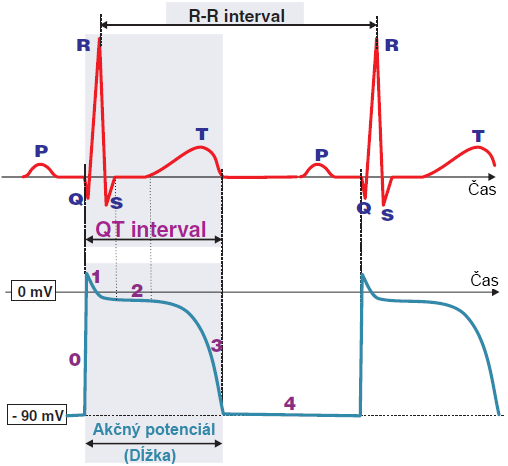
\includegraphics[scale=0.45]{img/action-potential-duration.png}
    \caption{Súvis akčného potenciálu srdcovej membrány a EKG krivky\cite{Blahút_2017}}
    \label{fig:action_potential_duration}
\end{figure}

\begin{itemize}
    \item \textbf{P-vlna} vzniká pri depolarizácii predsiení. Keďže svalová hmota predsiení je relatívne malá, na EKG krivke pri príslušných zvodoch pozorujeme malú oblú pozitívnu vlnu.
    \item \textbf{QRS komplex}, nazývaný aj komorový komplex, reprezentuje depolarizáciu komôr, obsahuje tri ostré za sebou idúce vlny. Z dôvodu väčšej svalovej hmoty je amplitúda vĺn komplexu výrazne vyššia. 
    \item \textbf{T-vlna} vzniká pri repolarizácii komôr, podobne ako pri P-vlne ide o malú oblú pozitívnu vlnu.\cite{Foster_2007}\cite{Bada2010}
\end{itemize}

%---------------------------------------------------------------
\subsection{Elektrická os srdečná}
%---------------------------------------------------------------

Aktivita srdca sa dá popísať mnohými vektormi, ktoré reprezentujú smer a silu elektrickej aktivity vznikajúcej v srdci. Samostatne vieme určiť napríklad aj elektrickú os srdcových komôr, pomocou vektorovej aritmetiky. "Konečný vektor, po všetkých sčítaniach, odčítaniach a zmenách smeru, reprezentuje elektrickú os srdcovej komory. Rovnako má každá vlna a každý segment tiež svoj príslušný vektor, vektor P-vlny, vektor S-T segmentu, alebo QRS vektor. EKG zachytáva tieto vektory počas toho, ako prechádzajú pod elektródou."\footnote{Pôvodné znenie: \textit{"That final vector, after all of the addition, subtraction, and direction changes, is known as the electrical axis of the ventricle. In the same way, each wave and segment has its own respective vector. There is a P-wave vector, a T-wave vector, an ST segment vector, and a QRS vector. The ECG is a measurement of these vectors as they pass under an electrode. "}}\cite{garcia201512}

Amplitúda vlny zobrazenej na EKG krivke závisí od uhlu, ktorý zviera vektor elektrického impulzu so zvodom. Ak je vektor paralelný s osou zvodu, amplitúda bude pri danom zvode maximálna, a klesá spolu s narastajúcim uhlom medzi nimi. V prípade, že sú na seba kolmé, na EKG krivke je viditeľná izoelektrická línia. Od orientácie vektoru elektrického impulzu zase záleží, či bude vlna na EKG krivke zobrazená ako pozitívna, alebo negatívna. 
\begin{itemize}
    \item \textbf{Pozitívna vlna} vzniká, ak sa pozitívny impulz hýbe smerom k elektróde. Keďže výsledkom depolarizácie je pozitívny potenciál, ak sa depolarizácia hýbe smerom k elektróde, vzniká pozitívna vlna. Opak platí pre repolarizáciu, pri ktorej vzniká negatívny potenciál - vlna bude pozitívna, ak sa hýbe smerom od elektródy.
    \item \textbf{Negatívna vlna} vzniká, ak sa pozitívny impulz hýbe smerom od elektródy. Z tvrdenia vyššie vyplýva, že ak sa depolarizácia hýbe v smere od elektródy, zaznamenaná vlna bude negatívna, a analogicky platí to isté, aj keď sa repolarizácia hýbe smerom od elektródy.\cite{garcia201512}\cite{Euan_Niebauer_2004}
\end{itemize}

\begin{figure}[H]
    \centering
    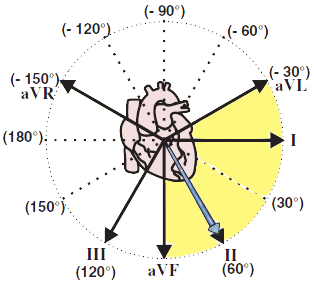
\includegraphics[scale=0.6]{img/normal-axis.png}
    \caption{Elektrická os srdečná\cite{Blahút_2017b}}
    \label{fig:axis}
\end{figure}

Fyziologicky je elektrická os srdečná orientovaná medzi -30° až + 90°, teda v ľavom dolnom kvadrante, ako je možné vidieť na obrázku \ref{fig:axis}. Keďže sa elektrický impulz v srdci šíri od pravej predsiene smerom k srdcovému hrotu, fyziologicky os približne zodpovedá orientácii srdca v hrudnej dutine.\cite{Bada2010} V prípade patológie označujeme elektrickú os ako derivovanú doprava, alebo derivovanú doľava.

%---------------------------------------------------------------
\subsection{Interpretácia EKG}
%---------------------------------------------------------------

Elektrokardiogram je kvôli dostupnosti a neinvazívnosti tejto metódy najčastejšie využívaná metóda v kardiológii. Dôkladnou analýzou záznamu je možné diagnostikovať rôzne srdcovo-cievne ochorenia, ako napríklad arytmie, či infarkt myokardu. Najdlhšou súvisle interpretovanou časťou v EKG krivke je QRS komplex, ktorý je tvorený zhlukom troch rovnomenných vĺn. Okrem samotných vĺn v rámci EKG krivky interpretujeme aj trvanie dvoch základných charakteristík - segmentov a intervalov.
\begin{itemize}
    \item \textbf{Segment} je časť izoelektrickej línie medzi jednotlivými vlnami, interpretujeme napríklad S-T alebo P-R segment.
    \item \textbf{Interval} je ohraničený začiatkom jednej a začiatkom druhej vlny. Tieto vlny môžu byť buď z toho istého srdečného cyklu, ako napríklad P-R alebo Q-T interval, alebo z dvoch po sebe idúcich cyklov, ako v prípade R-R intervalu.\cite{Wasilewski2011}
\end{itemize}

Pri interpretácii EKG sa kladie dôraz na dobu trvania a amplitúdy jednotlivých vĺn, segmentov, aj intervalov, pričom namerané hodnoty sa porovnávajú s fyziologickými. V tejto práci sa diagnostike srdcovo-cievnych ochorení venovať nebudeme, avšak v odbornej literatúre je možné nájsť veľké množstvo relevantných informácií k tejto téme.\cite{Wasilewski2011}\cite{Bada2010}\cite{Foster_2007}


%---------------------------------------------------------------
\section{Artefakty v EKG}
%---------------------------------------------------------------

Artefakty sú definované ako nežiaduce signály, alebo interferencie, ktoré nesúvisia s elektrickou aktivitou srdca a môžu viesť k nesprávnej interpretácii skutočného EKG signálu. Pochádzajú z rôznych zdrojov fyziologického, technického, alebo environmentálneho pôvodu. Keďže sú artefakty súčasťou zaznamenaného EKG signálu, izoelektrická línia alebo jednotlivé vlny pôsobia skreslené, čo môže viesť k nesprávnej diagnostike. Niektoré artefakty môžu simulovať klinicky významné arytmie, ako napríklad fibriláciu predsiení alebo komorovú tachykardiu. Hlavným úskalím je, že veľkú časť týchto artefaktov nie je možné odstrániť bez straty dôležitej informácie. 

Jedným z možných zdrojov artefaktov je chybné zapojenie elektród. Artefaktom tohto pôvodu sa ďalej nebudeme venovať, iba pre úplnosť spomenieme, že môžu spôsobiť prevrátený alebo inverzný signál pri postihnutých zvodoch.\cite{PrezRiera2017}\cite{Littmann2021} V nasledujúcej časti práce si popíšeme najbežnejšie artefakty, so zameraním na tie spôsobené fyzickou činnosťou. 

Príklad EKG krivky, na ktorej je zaznamenaný fyziologický sínusový rytmus, bez znečistenia artefaktmi, je možné vidieť na obrázku \ref{fig:sinus}.

\begin{figure}[H]
    \centering
    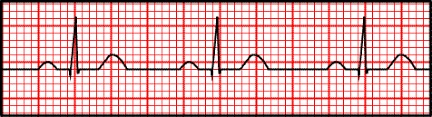
\includegraphics[scale=0.75]{img/sinus.jpg}
    \caption{Sínusový rytmus\cite{Mauvila_2018}}
    \label{fig:sinus}
\end{figure}

%---------------------------------------------------------------
\subsection{Kolísanie izoelektrickej línie}
%---------------------------------------------------------------

\begin{figure}[H]
    \centering
    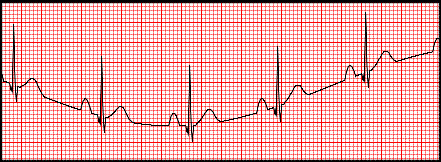
\includegraphics[scale=0.7]{img/baseline.jpg}
    \caption{Kolísanie izoelektrickej línie\cite{Mauvila_2018}}
\end{figure}

Ide o nízkofrekvenčný artefakt prejavujúci sa v EKG signáli ako postupný posun izoelektrickej línie v čase. Kolísanie izolínie môže pochádzať z rôznych zdrojov, často ide o respiračný artefakt spôsobený pohybom hrudníka pri dýchaní. Nedostatočný kontakt elektródy s kožou, prípadne nesúlad impedancií, môže spôsobiť kolísanie keď elektrický signál narazí na odpor na rozhraní koža-elektróda. Častým zdrojom je aj mimovoľný pohyb elektród spôsobený nedostatočnou fixáciou ku koži.\cite{Romero2018} Pri zaznamenávaní EKG signálu je potrebné na tieto skutočnosti myslieť, a snažiť sa eliminovať vyššie spomenuté zdroje čo najviac, ako sa dá, nie vždy je to však možné.

Medzi najpoužívanejšie metódy odstránenia kolísajúcej izolínie patria analógové alebo digitálne filtre s konečnou alebo nekonečnou odozvou, ktoré sú schopné selektívne prepúšťať alebo tlmiť špecifické frekvenčné zložky signálu. Analógové filtre sú zabudované priamo v zariadení snímajúcom EKG, kde filtrujú signál ešte pred digitalizáciou. Keďže ide o nízkofrekvenčný artefakt, využívajú sa filtre typu horná prepusť, ktoré prepúšťajú frekvencie vyššie ako stanovená hranica a tlmia nižšie. Porovnanie efektívnosti týchto filtrov je možné nájsť v odbornej literatúre, pričom sa kladie dôraz na čo najmenšiu stratu informácie v pôvodnom EKG signáli.\cite{Romero2018}\cite{Kaur2011}

%---------------------------------------------------------------
\subsection{Sieťové rušenie}
%---------------------------------------------------------------

\begin{figure}[H]
    \centering
    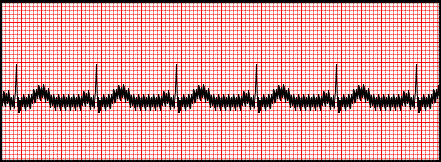
\includegraphics[scale=0.7]{img/acinterference.jpg}
    \caption{Sieťové rušenie\cite{Mauvila_2018}}
\end{figure}

Sieťové rušenie je často pozorovaný artefakt, zdrojom ktorého je striedavý prúd. Ide o rušenie s frekvenciou 50 Hz\footnote{Na území Európy sa štandardne elektrické zariadenia napájajú na striedavý prúd s frekvenciou 50 Hz, v iných častiach sveta je to často 60 Hz.}, ktoré sa prejavuje ako periodické fluktuácie v podobe špičiek superponovaných na skutočnej EKG krivke. Tento artefakt môže vznikať ako dôsledok elektromagnetickej väzby medzi elektrickými zvodmi, prípadne v dôsledku nedostatočného uzemnenia.\cite{Huhta1973} "Prítomnosť iných elektrických zariadení v miestnosti, kde sa zaznamenáva EKG, môže spôsobiť záznamy s viditeľným elektrickým rušením. V takýchto prípadoch by mali byť všetky zariadenia, ktoré môžu rušiť EKG signál, vypnuté. Medzi takéto zariadenia patria mobilné telefóny vo vzdialenosti menšej ako 25 cm od zariadenia zaznamenávajúceho EKG, elektrické lôžka, či chirurgické alebo fluorescenčné lampy."\footnote{Pôvodné znenie: \textit{"The presence of other electrical devices in the room where the ECG is being conducted may cause recordings with electrical inter- ference. In such cases, any device that may interfere with the ECG signal should be turned off: these include cell phones within 25 cm of the ECG sensor module, electrical beds, surgical and fluorescent lamps."}}\cite{PrezRiera2017}

Zabezpečenie správneho uzemnenia EKG zariadenia a tienenia káblov pred elektromagnetickým rušením,  znižuje pravdepodobnosť výskytu artefaktov spôsobených sieťovým rušením. Navyše majú systémy na monitorovanie EKG v sebe opäť často integrované analógové filtre, ktoré tento artefakt potláčajú. Keďže ide o opakované rušenie so známou frekvenciou, najčastejšie sa využívajú na jeho filtráciu hrebeňové filtre\footnote{Často uvádzané aj v pôvodnom anglickom znení ako \textit{notch filtre.}}, ktoré sú schopné potláčať konkrétne frekvencie. Filtrovanie je samozrejme možné vykonať aj po digitalizácii, kde je postup rovnaký, využívajú sa aj iné varianty pásmovej zádrže, ako napríklad Butterworthov filter.\cite{Gilani2018}

%---------------------------------------------------------------
\subsection{Pohybové artefakty}
%---------------------------------------------------------------

\begin{figure}[H]
    \centering
    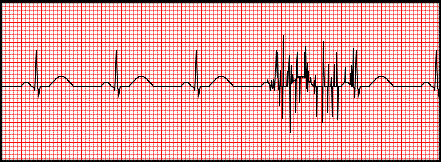
\includegraphics[scale=0.7]{img/tremor.jpg}
    \caption{Pohybový artefakt\cite{Mauvila_2018}}
\end{figure}

Pohybové artefakty sú najväčším problémom práve pri záťažovom testovaní, keďže vznikajú pri fyzickej aktivite. Zdrojom týchto artefaktov sú samotné nárazy spôsobené pohybom, zmena kontaktu medzi kožou a elektródou, či zmena impedancie na rozhraní koža-elektróda.\cite{Kirst2011} Špecifickým typom pohybového artefaktu sú myopotenciály, ktoré vznikajú kvôli svalovým kontrakciám,  prítomným pri pohybovej aktivite. 

Odstránenie pohybových artefaktov je najväčšou výzvou spomedzi spomínaných EKG artefaktov. Dôvodom je, že frekvenčné spektrum týchto artefaktov sa do významnej miery prekrýva so spektrom EKG, takže odstránenie bez straty dôležitej informácie nie je možné.\cite{Li2020} "Pohybové artefakty môžu produkovať signály s veľkou amplitúdou, ktoré pripomínajú P-vlny, T-vlny, či QRS-komplex. Sú prítomné počas ambulantného monitorovania a záťažových testov. Z klinického hľadiska môžu viesť k stanoveniu nesprávnej diagnózy, alebo oneskoreným či nevhodným rozhodnutiam týkajúcich sa liečby. Efektívne potlačenie pohybového artefaktu je v klinickom prostredí zatiaľ nevyriešeným problémom."\footnote{Pôvodné znenie: \textit{"Motion artifact can produce large amplitude signals in the ECG and can resemble the P, QRS, and T waveforms of the ECG. Motion artifact is prevalent during ambulatory monitoring and treadmill stress testing. From the clinical standpoint, motion artifact can result in misdiagnosis and may lead to delayed or inappropriate treatment decisions. Effective reduction of motion artifact is an unsolved problem in the clinical setting."}}\cite{Tong} Aj keď existujú postupy, akými sa dajú pohybové artefakty potlačiť, napríklad adaptívnym filtrovaním, kedy sa parametre filtru dynamicky menia\cite{Kirst2011}\cite{Tong}, tieto riešenia často nie sú dostatočné. 

V tejto práci sa však nebudeme zaoberať filtráciou pohybových artefaktov, ale ich automatickou detekciou. Dôvodom je, že pri dlhodobom terénnom monitorovaní, ktorého sa naša práca týka, je žiadúce tieto úseky identifikovať a následne od nich signál očistiť - teda segmenty znečistené pohybovými artefaktami zahodiť.


%---------------------------------------------------------------
\section{Automatická detekcia artefaktov v EKG}
%---------------------------------------------------------------

Problém detekcie pohybových artefaktov, ktorým sa táto práca zaoberá, je vo svojej podstate problém detekcie anomálií. V našom prípade anomálie nebudú predstavovať poruchy srdcového rytmu, ale samotné artefakty. Na rozdiel od detekcie anomálií sa detekcia pohybových artefaktov nezaoberá iba identifikáciou nesprávnych vzorov či deviácií od stanovenej normy, ale zaoberá sa aj posudzovaním kvality signálu.\footnote{Tento problém je v anglickej literatúre možné nájsť pod pojmom \textit{signal quality assessment} (SQA).} Práve kvalita signálu je rozhodujúca pri ďalšom spracovaní a interpretácii EKG záznamu.

Všetky z uvedených artefaktov sú ľahko identifikovateľné pomocou vizuálnej inšpekcie, zaujímavým aspektom tohto problému je však \textit{automatická} detekcia, s ktorou majú tradičné metódy spracovania signálu často problém. Práve to, že tradičné metódy na automatickú detekciu pohybových artefaktov nestačia, je motiváciou skúmať v tejto práci metódy založené na umelej inteligencii.

%---------------------------------------------------------------
\subsection{Tradičné metódy spracovania signálu}
%---------------------------------------------------------------

Medzi tradičné metódy spracovania signálu budeme radiť metódy zaoberajúce sa štatistickou analýzou a rôzne techniky dekompozície signálu. Patrila by sem samozrejme aj analógová a digitálna filtrácia, ako už ale bolo vyššie spomenuté, kvôli prekrývajúcemu sa frekvenčnému spektru tento prístup nie je v prípade pohybových artefaktov účinný. V krátkosti uvedieme dve metódy tradičného spracovania signálov vyskytujúce sa v literatúre v kontexte posudzovania kvality signálu a detekcie artefaktov.

\begin{itemize}
    \item \textbf{Analýza nezávislých komponentov (ICA)} je metóda dekompozície signálu, ktorá dokáže rozložiť signál na množinu štatisticky nezávislých komponentov, predpokladom je, že dáta pochádzajú z iného ako Gaussovského rozdelenia. Tým, že pohybové artefakty a EKG signál pochádzajú zo štatisticky nezávislých zdrojov, táto metóda je schopná ich odseparovať.\cite{Milanesi2007}
    \item \textbf{Vlnková transformácia} funguje na podobnom princípe ako Fourierova transformácia, ale je vhodnejšia na detekciu pohybových artefaktov. Dôvodom je, že nerozkladá signál iba na harmonické zložky, ktoré pretrvávajú po celú dobu signálu, ale dokáže nájsť zložky definované nie len špecifickou frekvenciou, ale aj časom. Analýzou získaných vlnkové koeficienty sa dajú odhaliť časovo-frekvenčné charakteristiky pohybového signálu.\cite{Bhoraniya2014}  
\end{itemize}

Veľkou nevýhodou použitia tradičných metód na detekciu pohybových artefaktov je, že sa často spoliehajú na analýzu špecifických charakteristík vstupných dát. Kvôli tomu nie sú schopné dobre generalizovať naprieč rôznymi množinami dát, ktoré napríklad nemusia byť zaznamenané za tých istých podmienok. Toto je veľký problém práve preto, lebo pohybové artefakty sú veľmi variabilné, závisia od vykonávanej aktivity, ale aj od polohy a typu elektród. Ďalšou významnou nevýhodou je časová náročnosť výpočtu. Metódy umelej inteligencie, ktoré budú bližšie opísané v nasledujúcich kapitolách, sú typicky vo fáze učenia tiež časovo náročné, avšak pri predikcii už nie. Výhodou tradičných metód je dobrá interpretovateľnosť výsledkov, tá sa však dá lepšie aplikovať na analýzu vlastností pohybových artefaktov než na samotnú automatickú detekciu.

%---------------------------------------------------------------
\subsection{Umelé neurónové siete (ANN)}
%---------------------------------------------------------------

Aby sme mohli ďalej rozoberať konkrétne architektúry neurónových sietí, ktoré sa využívajú na analýzu signálov, alebo časových rád, potrebujeme uviesť krátky opis umelých neurónových sietí ako takých. Sú to výpočtové modely, ktoré svojou štruktúrou a princípom pripomínajú ľudský nervový systém, čím sa snažia nadobudnúť schopnosť \textbf{generalizovať} a riešiť komplexné problémy. 

Základnou stavebnou jednotkou neurónovej siete je \textbf{neurón}, model ktorého je možné vidieť na obrázku \ref{fig:perceptron}. Tento model, ktorý sa nazýva \textbf{perceptrón}, sám o sebe slúži ako najjednoduchšia neurónová sieť, schopná riešiť úlohu binárnej klasifikácie.\cite{Minsky1969-vq} 

\begin{figure}[H]
    \centering
    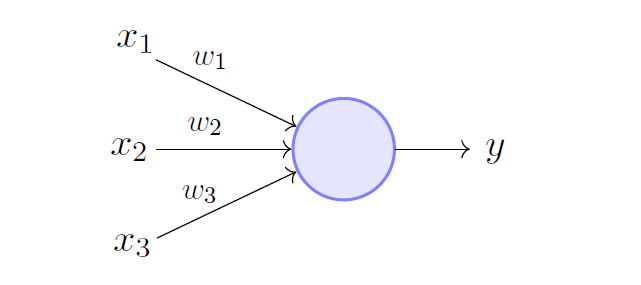
\includegraphics[scale=0.3]{img/perceptron.png}
    \caption{Jednoduchý perceptrón\cite{Minsky1969-vq}}
    \label{fig:perceptron}
\end{figure}

Model neurónu obsahuje \textit{n} vstupov, ktoré značíme \textit{x\textsubscript{1}} až \textit{x\textsubscript{n}}, k ním prislúchajú váhy \textit{w\textsubscript{1}} až \textit{w\textsubscript{n}}. Výstup neurónu \textit{y} je definovaný vzorcom \ref{eq:1}, dostávame ho ako lineárnu kombináciu vektoru vstupov \textit{\( \Bar{x} \)} a vektoru váh \textit{\( \Bar{w} \)}. \textit{T} predstavuje prah, pri ktorom je neurón aktivovaný a \textit{f} definuje \textbf{aktivačnú funkciu}. 

\begin{equation} 
    \label{eq:1}
    y = f(\sum_{i=0}^{n} w_i x_i - T)
\end{equation}

Tá zavádza do modelu žiadanú nelinearitu, keďže máloktorý reálny problém je lineárne separovateľný, a mala by byť spojitá a diferencovateľná kvôli učeniu pomocou gradientných optimalizačných algoritmov. Častou voľbou pri binárnej klasifikácii je sigmoida \ref{eq:2} a pri klasifikácii do viacerých tried funkcia softmax \ref{eq:3}. Softmax narozdiel od sigmoidy dáva na výstup rozdelenie pravdepodobnosti naprieč \textit{K} triedami, pričom zaručuje, že súčet jednotlivých pravdepodobností bude rovný jednej.\cite{Zou2008}\cite{yegnanarayana2009artificial}\cite{mehrotra1997elements}

\vspace{5pt}
\noindent
\begin{minipage}[t]{.45\textwidth}
    \begin{equation} 
        \label{eq:2}
        \sigma(x) = \frac{1}{1 + e^{-x}}
    \end{equation}
\end{minipage}
\hfill
\begin{minipage}[t]{.45\textwidth}
    \begin{equation} 
        \label{eq:3}
        softmax(x_i) = \frac{e^{x_i}}{\sum_{j=1}^{K} e^{x_j}}
    \end{equation}
\end{minipage}
\vspace{5pt}

Z hľadiska prepojenia neurónov poznáme dva rôzne druhy neurónových sietí - \textbf{dopredné a spätnoväzebné}. V dopredných sieťach sa informácia šíri iba jedným smerom, zatiaľ čo v spätnoväzebných sú umožnené aj spätné prepojenia, príkladom sú rekurentné neurónové siete.
Jednotlivé neuróny sú usporiadané do lineárnych polí, tie sa nazývajú \textbf{vrstvy}. Poznáme tri rôzne typy vrstiev z hľadiska usporiadania a to vstupné, skryté a výstupné. 
\begin{itemize}
    \item \textbf{Vstupná vrstva} je zodpovedná za inicializáciu vstupných dát do siete. Počet neurónov vo vstupnej vrstve je rovný rozmeru vstupných dát. Do každého neurónu príde na vstup jeden príznak, alebo v našom prípade jeden prvok z časovej rady reprezentujúcej EKG. 
    \item \textbf{Skrytá vrstva} je ktorákoľvek vrstva, ktorá sa nachádza medzi vstupnou a výstupnou, s ich narastajúcim počtom označujeme umelú neurónovú sieť ako \textbf{hlbokú}. Tieto vrstvy môžu mať rôzne topológie, ktoré je potrebné optimalizovať pre konkrétny problém, poznáme napríklad plne prepojené, alebo konvolučné vrstvy.
    \item \textbf{Výstupná vrstva} je poslednou vrstvou neurónovej siete, jej rozmer je určený požadovaným výstupom. V prípade klasifikačných úloh, akou je aj detekcia artefaktov, bude výstupná vrstva obsahovať počet neurónov rovný počtu tried. Každý neurón bude na záver obsahovať pravdepodobnosť, s ktorou daný vstup patrí do tejto triedy.
\end{itemize}

V tejto práci budeme využívať učenie s učiteľom, takže vstupné dáta budú mať priradené výstupné hodnoty, ktoré sa snaží neurónová sieť s čo najväčšou presnosťou naučiť predikovať. Optimalizáciu vektorov váh \textit{\( \Bar{w} \)} tak, aby neurónová sieť dosiahla čo najpresnejšie predikcie, nazývame \textbf{učenie} neurónovej siete. V skutočnosti ide o iteratívne hľadanie minima \textbf{stratovej funkcie}. Na začiatku sú vektory váh inicializované náhodne, prípadne je možné na ich inicializáciu použiť heuristiku. V každej iterácii trénovania, teda \textbf{epoche}, sa najskôr vykoná \textbf{dopredný krok}, kedy sa vstupné dáta propagujú sieťou až na výstup. Následne sa vypočíta strata modelu, porovnaním predikcií so správnymi hodnotami. Ako stratová funkcia pri klasifikačných úlohach sa často volí kategorická krížová entropia, ktorá je zadefinovaná ako \ref{eq:4}, kde \textit{c} značí počet tried.

\begin{equation} 
    \label{eq:4}
    L = -\sum_{i=1}^{c} y_i log(\hat{y_i})
\end{equation}

Vypočítaná strata modelu sa následne pomocou algoritmu \textbf{spätného šírenia chyby} propaguje neurónovou sieťou späť. Počas tohto kroku sa postupne počítajú gradienty stratovej funkcie vzhľadom k jednotlivým parametrom. Ako posledný krok jednej epochy sa vykoná aktualizácia váh modelu, kedy sa pomocou gradientnej optimalizácie posunú ich hodnoty proti smeru gradientu, teda smerom k minimu funkcie.\cite{Zou2008}\cite{yegnanarayana2009artificial}\cite{mehrotra1997elements} Aktualizácia \textit{n}-tej váhy je definovaná vzťahom \ref{eq:5}, pričom \textit{\( \alpha \)} predstavuje hyperparameter \textbf{learning rate}, ktorý reguluje rýchlosť učenia. 

\begin{equation} 
    \label{eq:5}
    *w_n = w_n - \alpha(\frac{\delta L}{\delta w_n})
\end{equation}

Darji a spol.\cite{Darji2013} riešili v svojej publikácii problém podobný nášmu použitím umelých neurónových sietí. Pomocou algoritmu na synchronizáciu R-špičiek odhadli z dát zložku reprezentujúcu pohybový artefakt pri štyroch rôznych fyzických aktivitách. Následne zo získaných zložiek ešte extrahovali časové a frekvenčné príznaky, ktoré potom vložili na vstup umelej neurónovej siete s desiatimi skrytými vrstvami. Na výstupe predikovali typ pohybovej aktivity s presnosťou 89.07\%.

%---------------------------------------------------------------
\subsection{Konvolučné neurónové siete (CNN)}
%---------------------------------------------------------------

Konvolučné neurónové siete sú konkrétnym druhom umelých neurónových sietí, ktoré sú určené na spracovanie viac-dimenzionálnych dát, akými sú napríklad časové rady alebo obrazové dáta. Špeciálne vrstvy vykonávajú operáciu nazývanú konvolúcia, použitý filter sa nazýva \textbf{kernel}. Okno filtra sa postupne posúva cez dáta, pričom počíta jednotlivé skalárne súčiny, ktoré sa zapisujú na príslušnú pozíciu výslednej matice. Operácia konvolúcie je znázornená na obrázku \ref{fig:convolution}, kde je matica \textit{I} konvolvovaná s kernelom \textit{K}. Okrem toho, že tieto vrstvy umožňujú hirearchickú extrakciu príznakov, slúžia aj na zníženie komplexnosti modelu, keďže nie sú plne prepojené.

\begin{figure}[H]
    \centering
    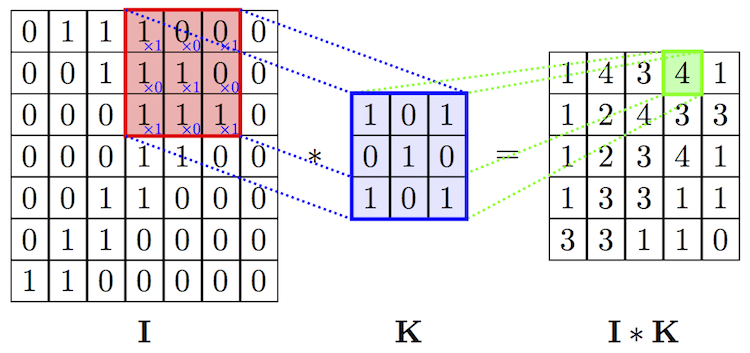
\includegraphics[scale=0.3]{img/convolution.png}
    \caption{Konvolúcia matice s kernelom\cite{mohamed2017}}
    \label{fig:convolution}
\end{figure}

Architektúra týchto sietí zahŕňa kombináciu plne prepojených, konvolučných a poolingových vrstiev.
\begin{itemize}
    \item \textbf{Konvolučné vrstvy}, ktoré vykonávajú vyššie popísanú operáciu, sú filtre, ktoré umožňujú neurónovej sieti extrahovať konkrétne informácie. Výsledkom aplikácie konvolúcie na dáta sú matice nazývané \textbf{aktivačné mapy}. Takto získané mapy je možné vizualizovať a analyzovať tak získané príznaky. 
    \item \textbf{Poolingové vrstvy}  redukujú rozmer vzniknutých máp, kedy sú susedné prvky zlúčené do jedného, pomocou matematických operácií ako sčítanie, alebo priemerovanie. Tieto vrstvy opäť redukujú komplexnosť siete a znižujú aj riziko preučenia.
    \item \textbf{Plne prepojené vrstvy} sú zodpovedné za integráciu informácií získaných v jednotlivých konvolučných vrstvách a následný výpočet predikcií.\cite{Sakib2019}\cite{Aloysius2017}\cite{Albawi2017}
\end{itemize}

Zhang a spol.\cite{Zhang2019} na klasifikáciu kvality EKG signálu využili kaskádu konvolučných neurónových sietí. Architektúra siete sa skladá z dvoch hlavných pod-sietí. Prvá klasifikuje signál do troch kategórií - pohybový artefakt, myopotenciál a signál s minimálnym rušením. Výstup z tejto pod-siete následne ide na vstup do druhej, ktorá ďalej klasifikuje pohybové artefakty a myopotenciály na mierne a závažné. Prvá pod-sieť sa skladá z troch samostatných sietí. Do jednej siete ide na vstup EKG signál očistený od šumu, do druhej vstupuje spektrogram signálu získaný pomocou krátkodobej Fourierovej transformácie, takže model zohľadňuje okrem časovej aj frekvenčnú zložku. Výstupy z oboch týchto sietí idú na záver na vstup do jedno-vrstvovej neurónovej siete obsahujúcej plne prepojenú vrstvu so softmax aktivačnou funkciou, ktorá výsledok klasifikuje do jednej z troch tried.

Zaujímavosťou tejto publikácie je aj to, že podrobne opisuje spôsob anotácie EKG dát. Dĺžka jedného segmentu bola zvolená ako 4 sekundy, s tým, že segment bol anotovaný podľa dominantného artefaktu. Artefakt bol segmentu priradený v prípade, že presahoval dĺžku 2 sekundy, závažnosť artefaktu bola zas odvodená od amplitúdy, relatívne k amplitúde R-špičky. \cite{Zhang2019} Využitie tejto metódy na monitorovanie v reálnom čase je diskutabilné, keďže výpočet spektrogramu môže byť časovo náročný.

%---------------------------------------------------------------
\subsection{Rekurentné neurónové siete (RNN)}
%---------------------------------------------------------------

Rekurentné neurónové siete sú ďalším typom umelých neurónových sietí, v tomto prípade ide o spätnoväzebné siete. Spätné väzby v tejto triede modelov umožňujú pamätať si informáciu a modelovať dáta obsahujúce časové závislosti. Pri analýze časových radov to znamená, že sú schopné efektívne riešiť problémy ako rozpoznávanie vzorov v dátach, či detekciu anomálií. 

Tradičné architektúry rekurentných neurónových sietí sa spoliehajú na spätné prepojenia, príkladom je napríklad plne-prepojená RNN, kde je každý neurón v skrytej vrstve napojený na všetky ostatné neuróny. Okrem toho medzi tradičné architektúry spadajú aj Elmanova a Jordanova sieť, oboje využívajú špeciálne kontextové bunky, ktoré sú napojené na vstup aj výstup buniek v skrytých vrstvách, čím modelujú prepojenie s predošlým krokom v čase. Všetky tieto architektúry ale zdieľajú dva problémy. Spolu s narastajúcou vzdialenosťou medzi časovými krokmi strácajú schopnosť pamätať si informáciu, takže nie sú vhodné na modelovanie dlhodobých časových závislostí.\cite{Staudemeyer2019} Druhým problémom je takzvaný miznúci gradient, kedy gradient propagovaný cez mnoho časových krokov začne exponenciálne klesať, následkom čoho sa váhy aktualizujú po veľmi malých krokoch, čo vedie k stagnácii trénovania.\cite{Hochreiter1998}   

Riešením oboch spomenutých problémov je novšia architektúra rekurentných neurónových sietí \textbf{LSTM} (Long Short-Term Memory). Táto architektúra využíva pamäťové LSTM bunky, ktoré majú v pamäti uložený vektor reprezentujúci stav bunky. Tok informácií dnu a von z tejto bunky je kontrolovaný pomocou troch brán, ktoré umožňujú zachytávať aj dlhodobé vzťahy v dátach.

\begin{itemize}
    \item \textbf{Vstupná brána} na základe aktuálneho vstupu a skrytého stavu určuje, ktorá časť vstupnej informácie sa uloží v pamäti.
    \item \textbf{Výstupná brána} na základe aktuálneho vstupu a aktualizovaného skrytého stavu určuje, aká časť uloženej informácie príde na výstup bunky.
    \item \textbf{Brána zabúdania} na základe aktuálneho vstupu a skrytého stavu určuje, ktorá časť vstupnej informácie bude ponechaná.\cite{Yu2019}
\end{itemize}

Špecifikom rekurentných neurónových sietí je to, že kvôli nutnosti propagácie chyby aj cez rekurentné prepojenia použitie štandardného trénovacieho algoritmu spätného šírenia chyby už nie je možné. Miesto toho sa najčastejšie využíva jeho rozšírená verzia, nazývaná \textbf{algoritmus spätného šírenia chyby v čase (BPTT).} "Na konci trénovacej sekvencie sa sieť rozvinie v čase a vypočíta sa chyba pre dvojice vstupov a výstupov pomocou zvolenej metriky. Následne sa táto chyba propaguje späť sieťou a vypočíta sa aktualizácia váh pre každý krok v čase. Na záver sa váhy v rekurentnej verzii siete aktualizujú ako súčet vypočítaných zmien naprieč všetkými krokmi."\footnote{Pôvodné znenie: \textit{"At the end of a training sequence, the network is unfolded in time. The error is calculated for the output units with existing target values using some chosen error measure. Then, the error is injected backwards into the network and the weight updates for all time steps calculated. The weights in the recurrent version of the network are updated with the sum of its deltas over all time steps."}}\cite{Yu2019} Ukážka rozvinutia rekurentnej neurónovej siete v čase \textit{t} je na obrázku \ref{fig:backpropagation}.

\begin{figure}[H]
    \centering
    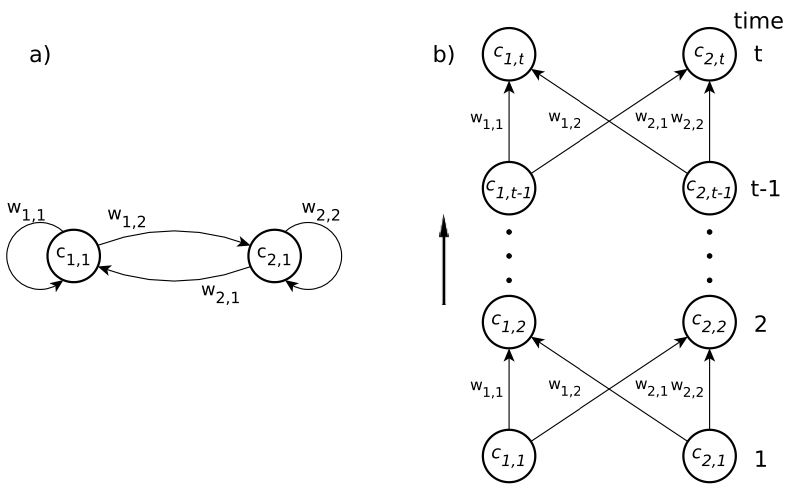
\includegraphics[scale=0.7]{img/backpropagation.png}
    \caption{Rozvinutie rekurentnej neurónovej siete v čase\cite{Yu2019}}
    \label{fig:backpropagation}
\end{figure}

Boljanić a spol.\cite{boljanic2022} sa v ich publikácii zaoberajú detekciou EKG artefaktov pomocou LSTM neurónových sietí. Dáta, na ktorých bola táto sieť trénovaná, úzko súvisia so zámerom našej práce - EKG signály z 1-zvodového systému boli zaznamenané od horských záchranárov počas zásahu. Signál bol rozdelený na 10 sekundové segmenty, a segment bol označený ako obsahujúci pohybový artefakt ak viac ako polovica segmentu obsahovala šum, kvôli ktorému sa nedal jasne detegovať QRS-komplex. Architektúra použitej siete sa skladá z obojsmernej LSTM vrstvy (BiLSTM), ktorej výstup ide na vstup plne prepojenej vrstvy so softmax aktivačnou funkciou. Po vyladení hyperparametrov bola táto rekurentná neurónová sieť schopná dosiahnuť presnosť 90.1\% na testovacích dátach. Hlavným obmedzením tohto prístupu je dlhé časové okno.

%---------------------------------------------------------------
\subsection{Support vector machines (SVM)}
%---------------------------------------------------------------

SVM je trieda modelov, ktorá sa najčastejšie používa na klasifikáciu dát. Problém, ktorý tieto modely riešia, je nájdenie \textbf{optimálnej separačnej nadroviny} - teda takej, ktorá maximalizuje vzdialenosť jednotlivých dátových bodov od nej. V prípade lineárne separovateľných dát je typicky možné nájsť nekonečne mnoho nadrovín separujúcich dáta. SVM operujú s myšlienkou, že čím ďalej dátové body od tejto nadroviny ležia, tým istejšia je klasifikácia a teda schopnosť modelu generalizovať narastá. Okolo nadroviny sa nachádza pásmo, v ktorom neležia žiadne body - to sa snažíme maximalizovať, hľadáme teda maximálny okraj\footnote{V Anglickom jazyku \textit{maximal margin}.}. Na definovanie nadroviny nám stačia body ležiace na tomto okraji, ktorých je typicky málo, takže sa pri výpočte pracuje s riedkou maticou, kvôli čomu je táto metóda výpočtovo efektívna. Tieto body, na ktorých závisí poloha nadroviny, nazývame \textbf{podporné vektory}\footnote{V Anglickom jazyku \textit{support vectors}.}. Na obrázku \ref{fig:margin} hrubá čiara reprezentuje optimálnu separačnú nadrovinu, a \textit{\( \gamma \)} definuje maximálny okraj.\cite{Cristianini_Scholkopf_2002}\cite{Suthaharan2016}

\begin{figure}[H]
    \centering
    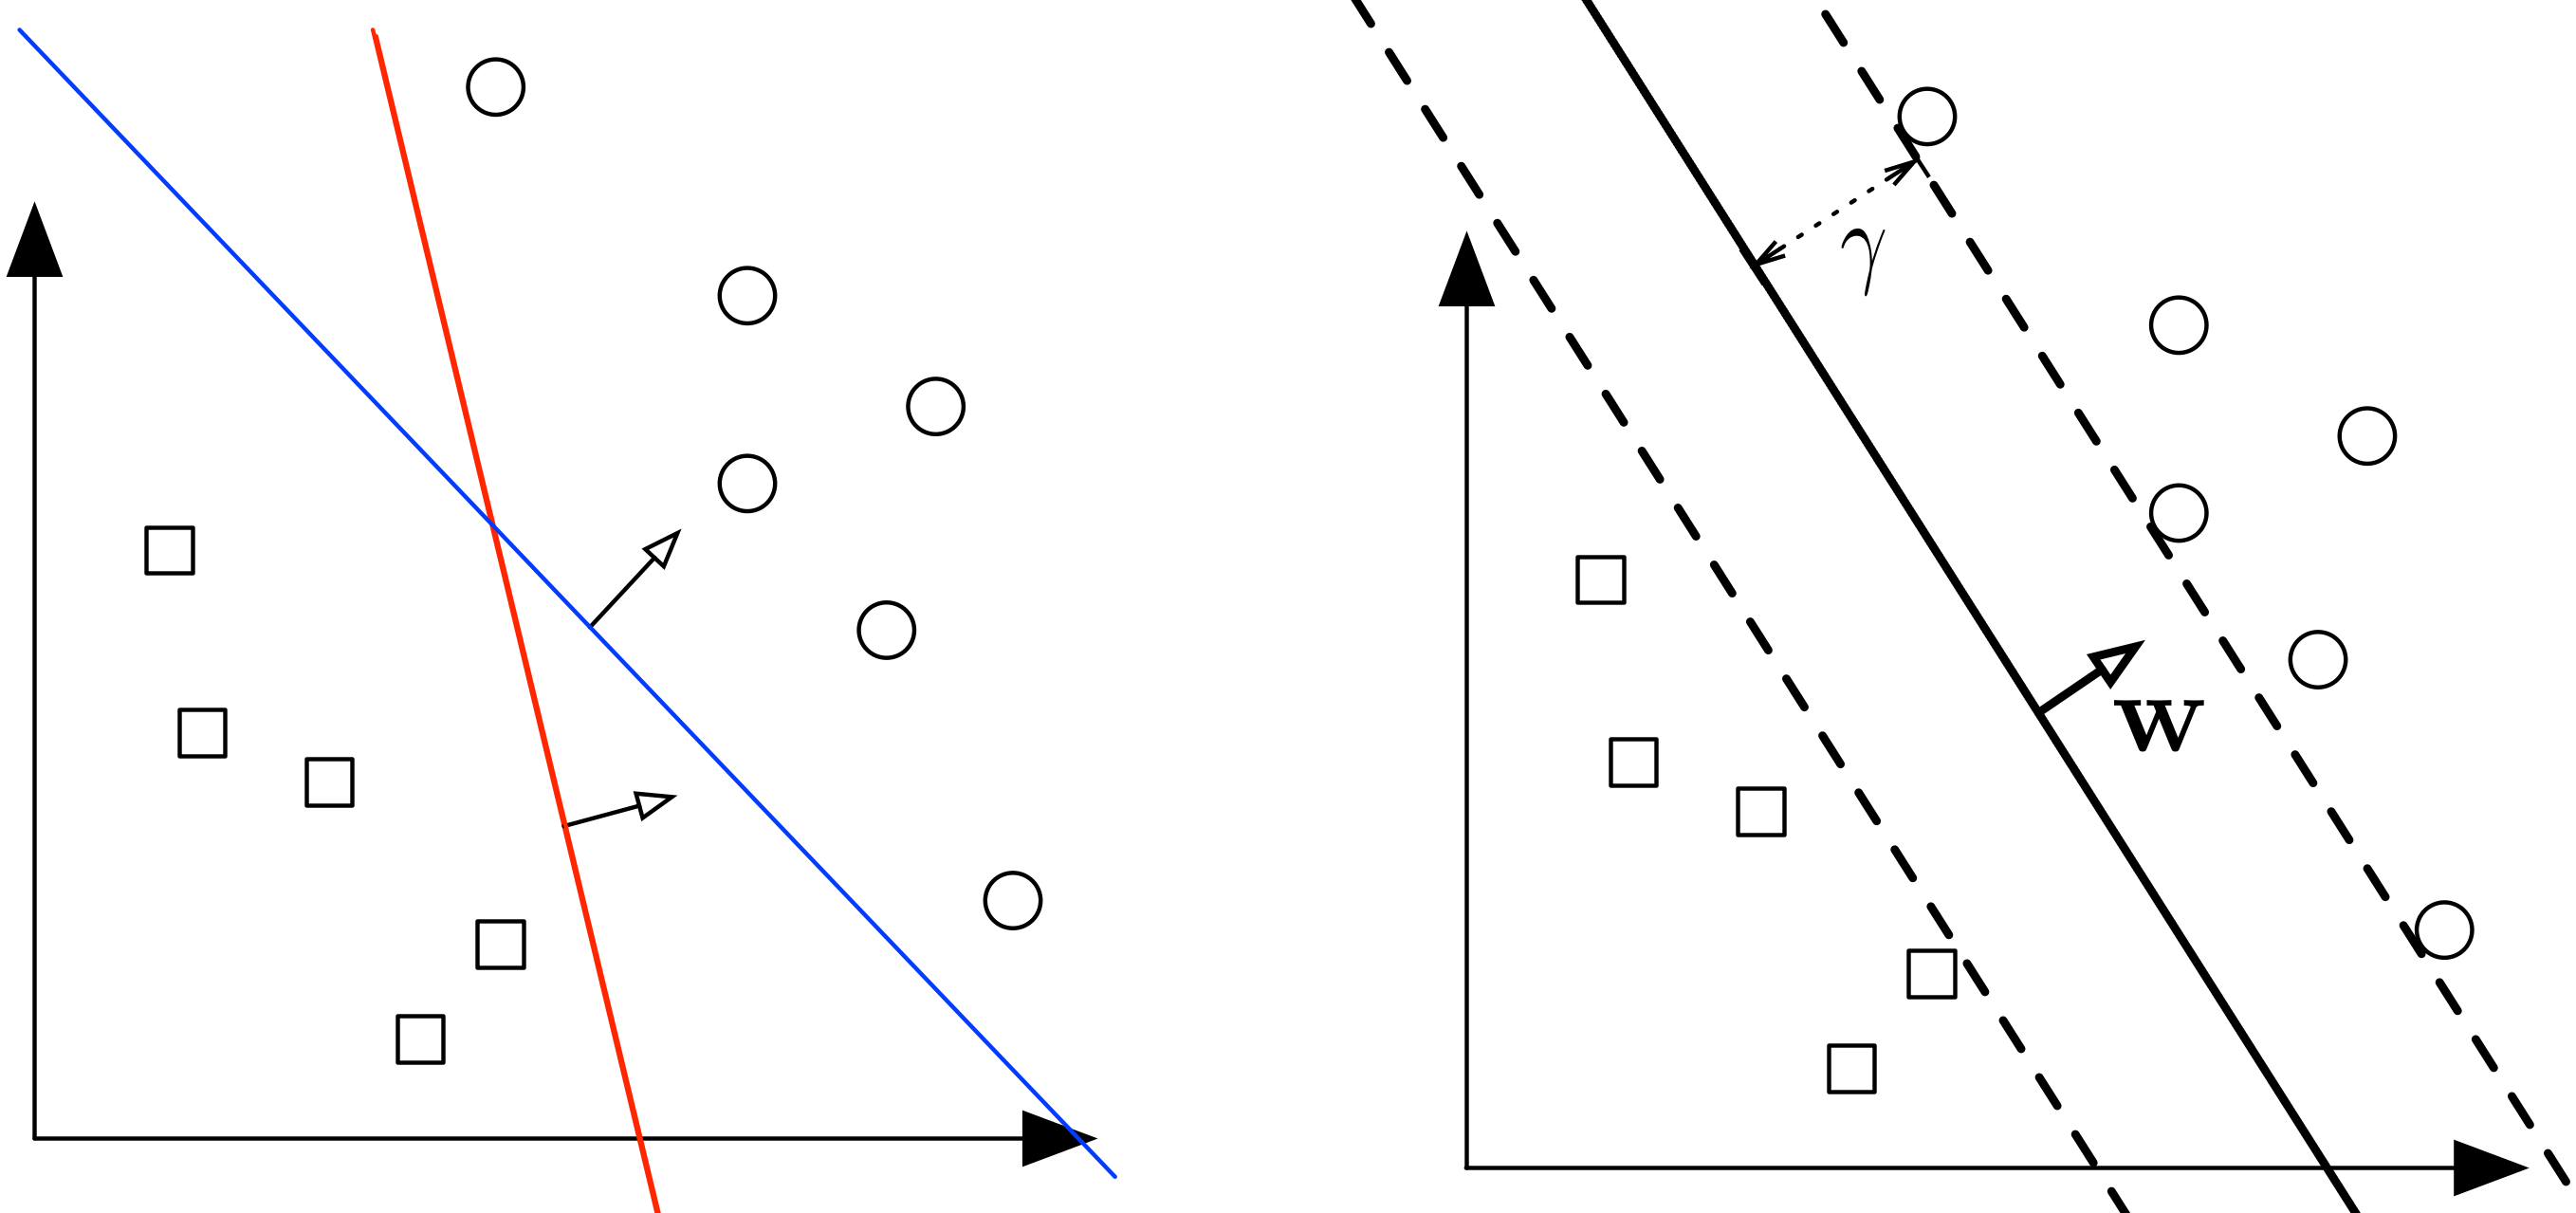
\includegraphics[scale=0.5]{img/margin.png}
    \caption{Optimálna separačná nadrovina\cite{Lecture_SVM}}
    \label{fig:margin}
\end{figure}

Ďalšou výhodou SVM modelov je, že v prípade, kedy dáta nie sú lineárne separovateľné, využívajú takzvaný \textbf{jadrový trik}, ktorý spočíva v tom, že pomocou \textbf{jadrovej funkcie} dáta transformuje do priestoru vyššej dimenzie, v ktorej už lineárne separovateľné sú. SVM modely taktiež nevyžadujú úplnú lineárnu separabilitu, v prípade, že sa dosiahnuť nedá, sa používa takzvaný mäkký okraj\footnote{V Anglickom jazyku \textit{soft margin}.}, ktorý umožňuje aj nesprávnu klasifikáciu. Tá je penalizovaná, čím prispieva k zmene predpisu nadroviny. Keďže transformácia dát do vyšších dimenzií vie byť výpočtovo veľmi náročná, jadrový trik využíva na túto transformáciu skalárne súčiny príznakov. Rôzne jadrové funkcie využívajú rôzne jadrá, dve často využívané sú \textbf{polynomiálne jadro} \ref{eq:6}, kde pre \textit{d}=1 dostávame \textbf{lineárne jadro}, a \textbf{Gaussovské (RBF) jadro} \ref{eq:7}, kde \textit{\( \gamma \)} reguluje šírku Gaussovskej krivky. Menšia hodnota znamená hladšiu rozhodovaciu hranicu, väčšia hodnota naopak členitejšiu.\cite{Cristianini_Scholkopf_2002}\cite{Suthaharan2016}

\vspace{5pt}
\noindent
\begin{minipage}[t]{.45\textwidth}
    \begin{equation} 
        \label{eq:6}
        K(x_i,x_j) = (x_i^{T} x_j)^{d}
    \end{equation}
\end{minipage}
\hfill
\begin{minipage}[t]{.45\textwidth}
    \begin{equation} 
        \label{eq:7}
        K(x_i,x_j) = {e^{-\gamma ||x_i - x_j||^{2}}}
    \end{equation}
\end{minipage}
\vspace{5pt}

Castaño a spol.\cite{Castao2017} v svojej publikácii skúmajú klasifikáciu pomocou SVM do dvoch tried - normálne EKG a znečistené pohybovým artefaktom. Použité dáta boli získané v kontrolovanom experimente podobne ako naše, avšak skúmaná bola iba jedna pohybová aktivita a to pohyb hornými končatinami. Namerané dáta boli rozdelené na segmenty o dĺžke 1.2 sekundy, korešpondujúce s jedným úderom srdca. Skúšali SVM s lineárnym aj polynomiálnym jadrom, ale najlepšie výsledky dosiahli pomocou Gaussovského jadra. Kher a spol.\cite{Kher2015} riešia problém klasifikácie rôznych pohybových aktivít - pohyby hornými končatinami, rotácie v páse a chôdza. Ich prístup je však odlišný v tom, že na klasifikáciu pomocou SVM nepoužívajú nespracovaný EKG signál, ale z neho extrahované príznaky pomocou rôznych transformácií, ako napríklad vyššie spomínanej vlnkovej transformácie. Aj keď pomocou Gaussovského jadra dosiali presnosť 95\%, kvôli využitiu transformácií však táto metóda nie je vhodná na klasifikáciu v reálnom čase.


%---------------------------------------------------------------
\chapter{Popis experimentu}
%---------------------------------------------------------------

%---------------------------------------------------------------
\section{Metodika experimentu}
%---------------------------------------------------------------

TODO

%---------------------------------------------------------------
\section{Použitý hardware}
%---------------------------------------------------------------

TODO

%---------------------------------------------------------------
\section{Použitý software}
%---------------------------------------------------------------

TODO

%---------------------------------------------------------------
\subsection{Vizualizácia a záznam EKG}
%---------------------------------------------------------------

\begin{figure}[H]
    \centering
    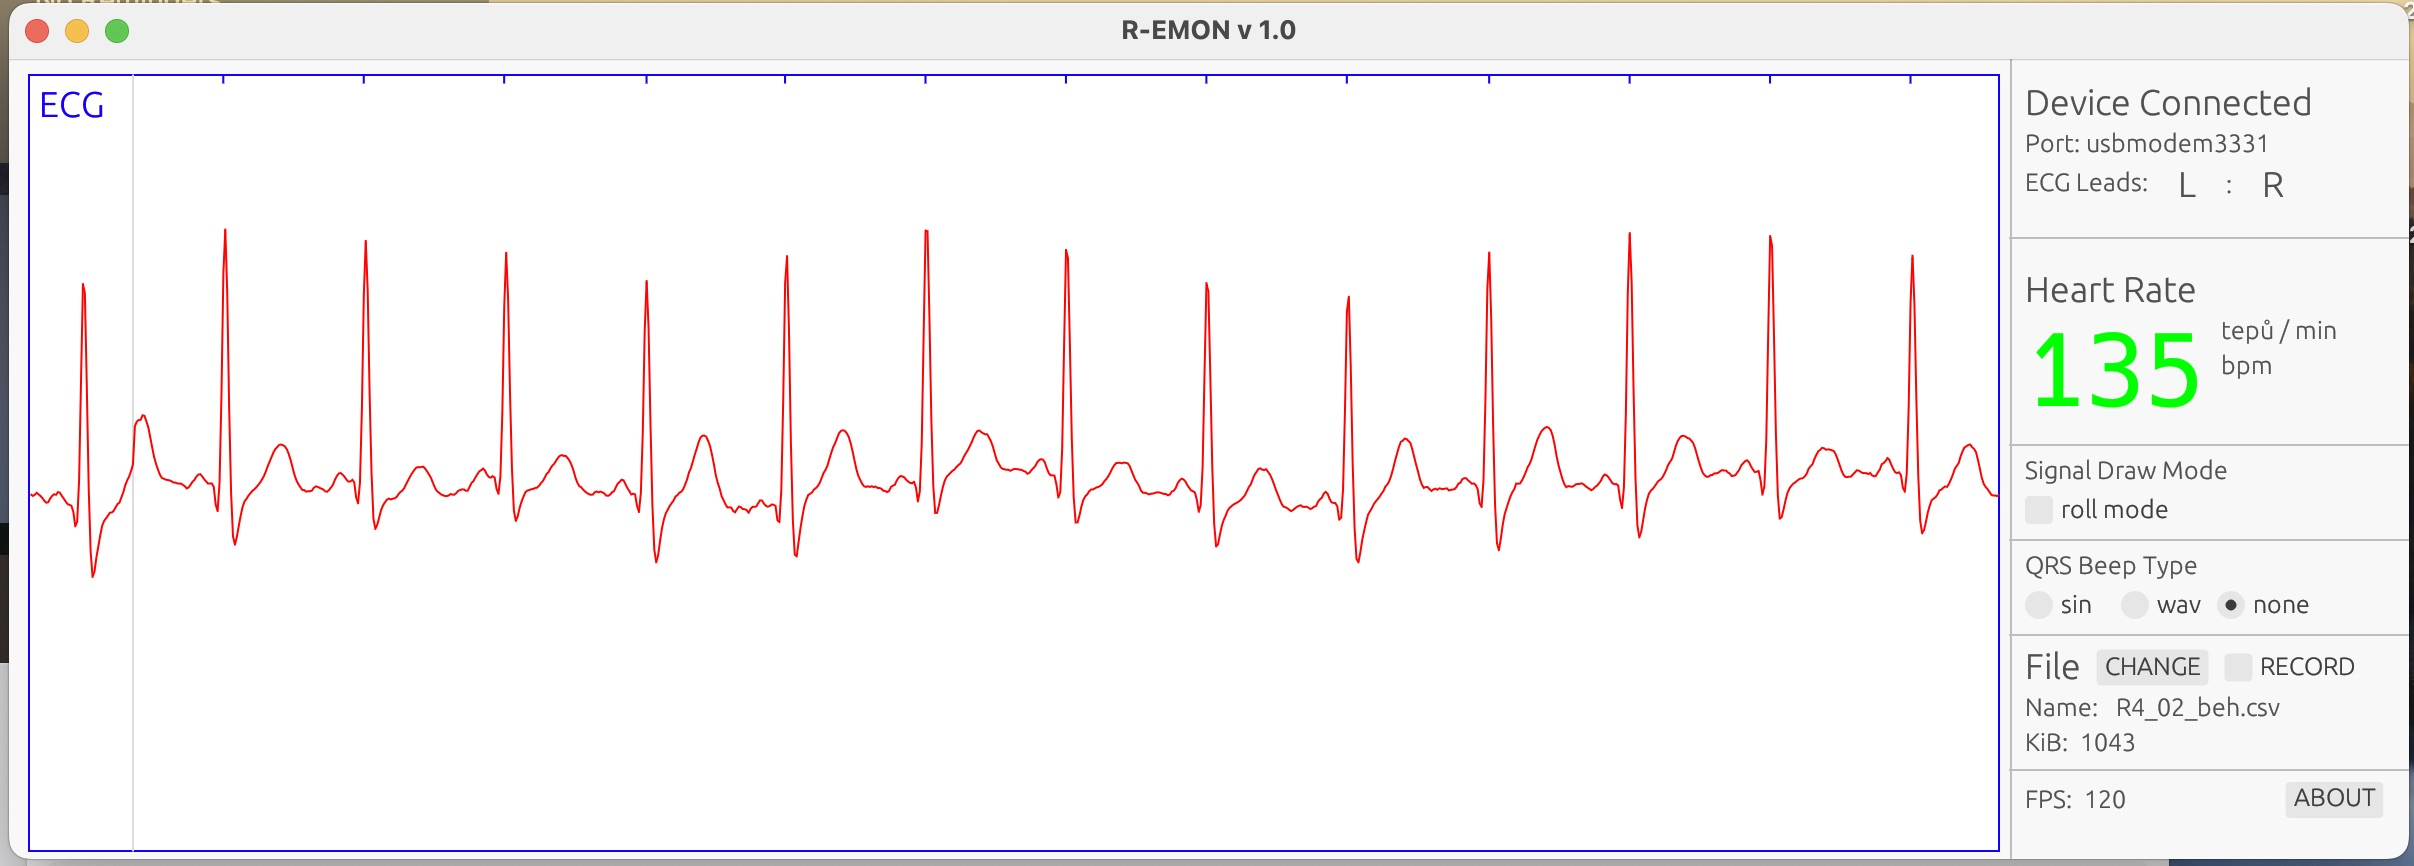
\includegraphics[scale=0.18]{img/ok.jpeg}
    \caption{Software na vizualizáciu a záznam EKG}
    \label{fig:SW_ok}
\end{figure}

%---------------------------------------------------------------
\subsection{Manuálna anotácia dát}
%---------------------------------------------------------------

Kvôli nutnosti manuálne anotovať namerané EKG dáta bolo na tento účel vytvorené jednoduché grafické rozhranie. Zdrojový kód je napísaný v programovacom jazyku \textbf{Python 3.0}, so staršími verziami nemusí byť kompatibilný. Užívateľské rozhranie bolo vytvorené pomocou \textbf{PyQt5}, ktoré poskytuje programátorské rozhranie medzi knižnicou na tvorbu grafických aplikácií Qt a jazykom Python. V tomto rozhraní je EKG krivka zobrazená na grafe vykreslenom pomocou knižnice \textbf{Matplotlib}. Kompletný zoznam knižníc potrebných na spustenie aplikácie je možné nájsť v zložke so zdrojovými kódmi v súbore \textit{requirements.txt}.

\begin{figure}[H]
    \centering
    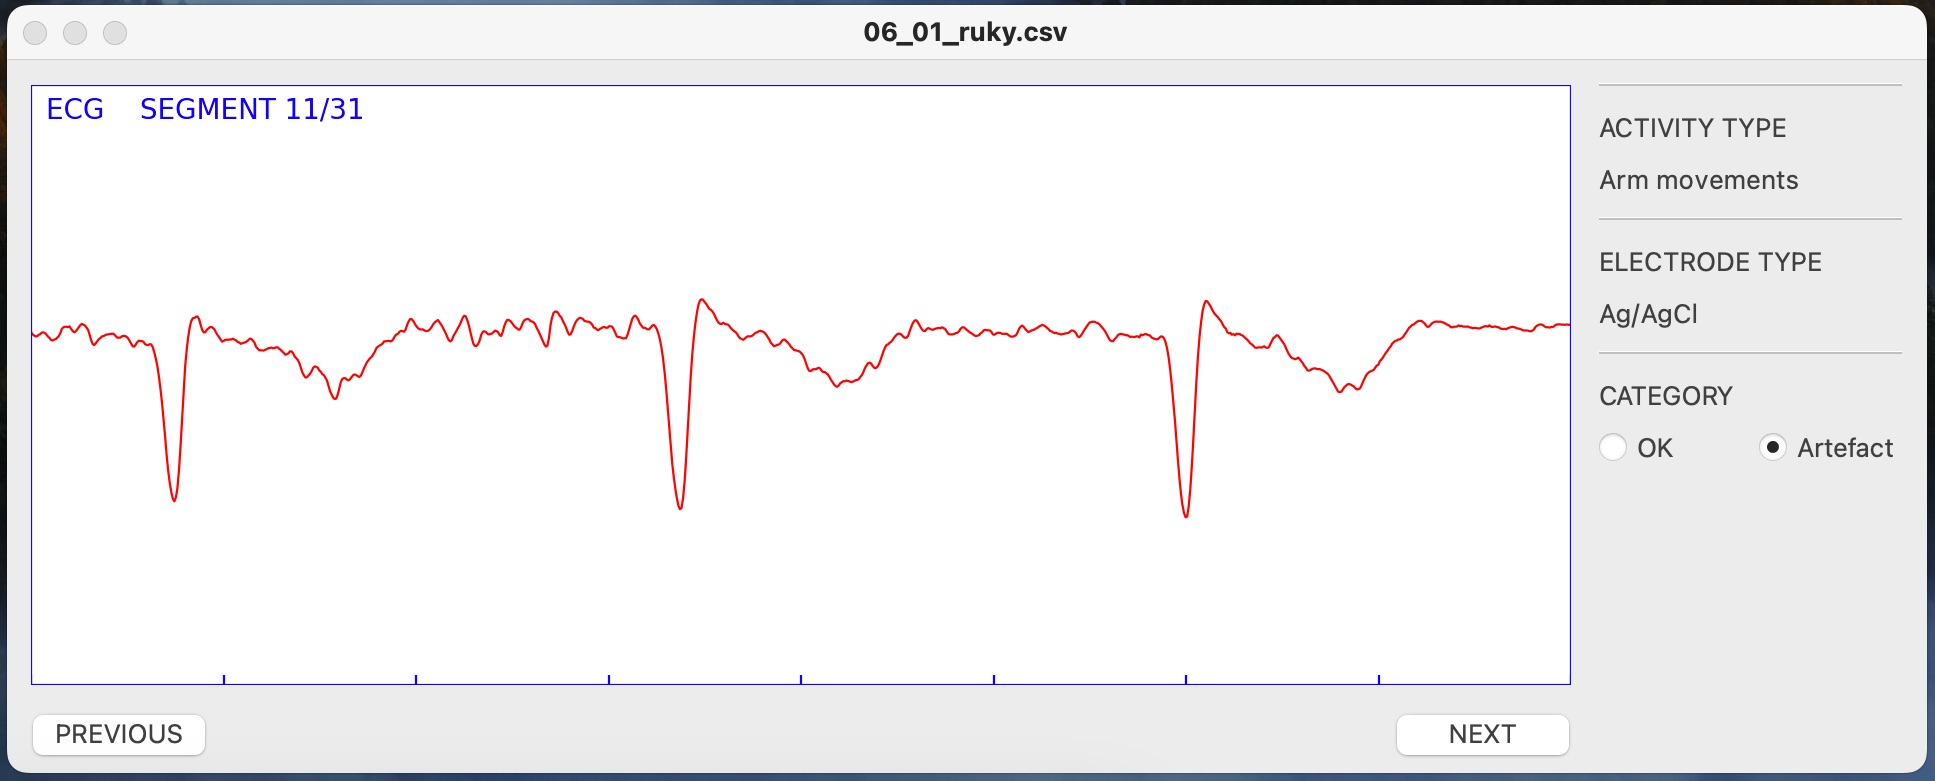
\includegraphics[scale=0.225]{img/annotation_sw.jpeg}
    \caption{Grafické rozhranie na manuálnu anotáciu EKG}
    \label{fig:SW_labels}
\end{figure}

Grafické rozhranie umožňuje navigáciu cez jednotlivé segmenty nameraného EKG signálu, pričom ich dĺžka je voliteľná. Na pohyb medzi jednotlivými segmentmi sa dajú použiť buď tlačidlá umiestnené pod oknom, v ktorom sa zobrazuje aktuálny segment, alebo pomocou ľavej a pravej šípky na klávesnici. V ľavom hornom rohu okna zobrazujúceho aktuálny segment sa nachádza číslo aktuálneho segmentu a ich celkový počet. V paneli na pravej strane okna sa nachádza typ pohybovej aktivity a použitých elektród, oboje sú odvodené od názvu súboru. V neposlednom rade sa tu nachádza aj prepínacie tlačidlo, ktorým sa anotuje daný segment ako obsahujúci artefakt, alebo čistý. Toto tlačidlo sa dá opäť ovládať priamo kliknutím, alebo sa dá na jeho prepínanie využiť medzerník na klávesnici. Pri otvorení vstupného súboru, ktorý chce používateľ anotovať, sa automaticky vytvorí výstupný \textit{.csv} súbor, rovnako sa pri zmene stavu prepínacieho tlačidla označujúceho artefakt tento súbor automaticky prepíše, explicitné ukladanie nie je nutné. 

Používateľské rozhranie je možné spustiť pomocou príkazu \textbf{python3 data\_labeler.py} z príslušnej zložky, a voliteľné parametre sú nasledovné:

 \noindent \textbf{data\_labeler.py [-l segment\_length] [-f sampling\_rate] [-s starting\_segment] input\_file}
 
\begin{tabbing}
    \indent \textbf{input\_file (str)} \quad\quad\quad\quad \= - názov vstupného súboru, musí byť súbor typu \textit{.csv}\\
                                                            \> nachádzajúci sa v zložke \textit{/data}\\
    \indent \textbf{segment\_length (int)}                  \> - dĺžka segmentu v sekundách, predvolená na 5 sekúnd\\
    \indent \textbf{sampling\_rate (int)}                   \> - vzorkovacia frekvencia vstupného súboru, predvolená na\\
                                                            \> 500 vzoriek za sekundu\\
    \indent \textbf{starting\_segment (int)}                \> - číslo počiatočného segmentu na zobrazenie, predvolené na\\
                                                            \> prvý segment\\
\end{tabbing}



%---------------------------------------------------------------
\chapter{Dátová sada}
%---------------------------------------------------------------

V nasledujúcej kapitole opíšeme štruktúru vzniknutej dátovej sady a v krátkosti aj rôzne štatistiky vyplývajúce z nej, ako napríklad súvis jednotlivých typov elektród s výskytom pohybových artefaktov. Dáta pre účastníkov experimentu sú členené do zložiek, pričom každý účastník ma svoju vlastnú, ktorá obsahuje všetky zaznamenané EKG dáta a k ním príslušné anotácie artefaktov. Experimentu za zúčastnilo \textbf{10 účastníkov}, pre každého je nameraných niekoľko záznamov dlhých približne jednu minútu - \textbf{5 rôznych fyzických aktivít} zaznamenaných pomocou \textbf{3 rôznych typov elektród}. Dostávame teda 15 záznamov pre každého účastníka, takže dokopy \textbf{150 minútových záznamov EKG}. Každý z týchto záznamov bol následne rozdelený na segmenty dlhé 2 sekundy, čím na záver získavame približne \textbf{4500 anotovaných segmentov}.

%---------------------------------------------------------------
\section{Demografia účastníkov experimentu}
%---------------------------------------------------------------

TODO

%---------------------------------------------------------------
\section{Štruktúra dát}
%---------------------------------------------------------------

EKG signál je zaznamenaný do súboru, ktorý obsahuje iba dva stĺpce - jeden pre časový údaj a druhý pre hodnotu signálu v danom čase, jeho štruktúru je možné vidieť v tabuľke \ref{tab:input}. Prvý aj druhý stĺpec obsahuje záznam vo forme časovej rady, v ukážke je zobrazených prvých 5 vzoriek záznamu.

\begin{table}[H]\centering
\caption[]{~Súbor s EKG záznamom}\label{tab:input}
    \begin{tabular}{c|c}
    	\textbf{timestamp} 	        & \textbf{value}   \tabularnewline \hline 
     	2024-03-26 15:04:53.249732  & 1698	           \tabularnewline \hline
     	2024-03-26 15:04:53.251727 	& 1874	           \tabularnewline \hline
        2024-03-26 15:04:53.253784 	& 2021	           \tabularnewline \hline
        2024-03-26 15:04:53.253784  & 2153	           \tabularnewline \hline
        2024-03-26 15:04:53.257780  & 2291	           \tabularnewline
    \end{tabular}
\end{table}

Pre správnu anotáciu typu pohybovej aktivity a zobrazenie druhu elektród v grafickom rozhraní je potrebné dodržať zaužívané názvoslovie súboru, ktoré je \textit{XX\_TYP-ELEKTRÓDY\_TYP-AKTIVITY.csv}. Typ pohybovej aktivity je kódovaný podľa tabuľky \ref{tab:labels_activity}, pričom neznáma hodnota sa uvádza v prípade, že názov súboru na príslušnom mieste neobsahuje ani jednu z uvedených aktivít. Typ použitých elektród je zas kódovaný podľa tabuľky \ref{tab:labels_electrode}.

\begin{table}[H]\centering
\caption[]{~Kódovanie pohybovej aktivity}\label{tab:labels_activity}
    \begin{tabular}{l|c}
    	\textbf{Pohybová aktivita}  & \textbf{Číselná hodnota}    \tabularnewline \hline 
     	Kľudová fáza                & 0	                          \tabularnewline \hline
     	Pohyby hornými končatinami 	& 1	                          \tabularnewline \hline
        Chôdza 4 km/h 	            & 2	                          \tabularnewline \hline
        Beh 8 km/h                  & 3	                          \tabularnewline \hline
        Drepy                       & 4	                          \tabularnewline \hline
        Neznáma                     & 5	                          \tabularnewline
    \end{tabular}
\end{table}

\begin{table}[H]\centering
\caption[]{~Kódovanie typu elektród}\label{tab:labels_electrode}
    \begin{tabular}{l|c}
    	\textbf{Typ elektród}  & \textbf{Číselná hodnota}     \tabularnewline \hline 
     	Ag/AgCl                & 1	                          \tabularnewline \hline
     	Chróm-niklel	       & 2	                          \tabularnewline \hline
        Textil	               & 3	                          \tabularnewline
    \end{tabular}
\end{table}

Názvoslovie súborov vytvorených pomocou grafického rozhrania na anotáciu dát je nasledovné - \textit{XX\_TYP-ELEKTRÓDY\_TYP-AKTIVITY\_DĹŽKA-SEGMENTU.csv}. Dĺžka segmentu je v názve uvedená kvôli tomu, aby sa dali odlíšiť anotácie tých istých vstupných súborov pre rôzne zvolené dĺžky segmentu. Súbory obsahujú stĺpec pre začiatočnú a koncovú pozíciu segmentu, typ aktivity a artefakt, ich štruktúra je zobrazená v tabuľke \ref{tab:output}. Príklad obsahuje anotáciu pre vstupný súbor obsahujúci záznam EKG signálu účastníka vykonávajúceho pohyb hornými končatinami. Vzorkovacia frekvencia je 500 vzoriek za sekundu a dĺžka segmentu 2 sekundy, pričom prvé dva segmenty obsahujú pohybový artefakt a nasledujúce dva nie. 

\begin{table}[H]\centering
\caption[]{~Výstupný súbor s anotovanými dátami}\label{tab:output}
    \begin{tabular}{c|c|c|c}
    	\textbf{start} & \textbf{end} & \textbf{activity} & \textbf{artifact}  \tabularnewline \hline 
     	0		       & 1000		  & 1	              & 0	               \tabularnewline \hline
     	1000	       & 2000	      & 1	              & 0	               \tabularnewline \hline
        2000	       & 3000	      & 1	              & 1	               \tabularnewline \hline
        3000	       & 4000	      & 1	              & 1	               \tabularnewline
    \end{tabular}
\end{table}



%---------------------------------------------------------------
\chapter{Zhodnotenie}
%---------------------------------------------------------------
